\section{Interface}
% The GUI of LuRaCs is divided into two panes with tabs containing the most important information for viewing and measuring spectra. These are supported by popup windows and dialogs for performing specific tasks, like loading files or performing a certain analysis method.
% \begin{figure}[H]
%     \centering
%     \includegraphics[width=0.95\linewidth]{images/interface/overview.jpg}
%     \caption{Enter Caption \\ second row}
%     \label{fig:placeholder}
% \end{figure}
\subsection{Primary Tabs}
\subsubsection{Spectrum}\label{sec:spectrum}
The spectrum tab shows spectra as a count histograms, retrieved from a connected detector or loaded from a compatible file. It can show several spectra combined in one plot or in separate tabs within the spectrum tab, see \autoref{fig:spectrum_with_cursor}. This can be changed under \texttt{Options -> Tabbed-/Combined Spectrum View} (then selecting the files or data to be shown).


Background spectra can be viewed as: \textit{Background overlay} and \textit{background subtract} or not at all: \textit{No background}. \textit{Background overlay} shows the background spectrum overlaid on top of the main (foreground) spectrum. \textit{Background subtract} subtracts the background, channel by channel, from the foreground spectrum. Note that this is a hard background subtraction and will thus effect spectrum ROI calculations. Both \textit{Background overlay} and \textit{Background subtract} are limited to show count rate values.

\begin{figure}[H]
    \centering
    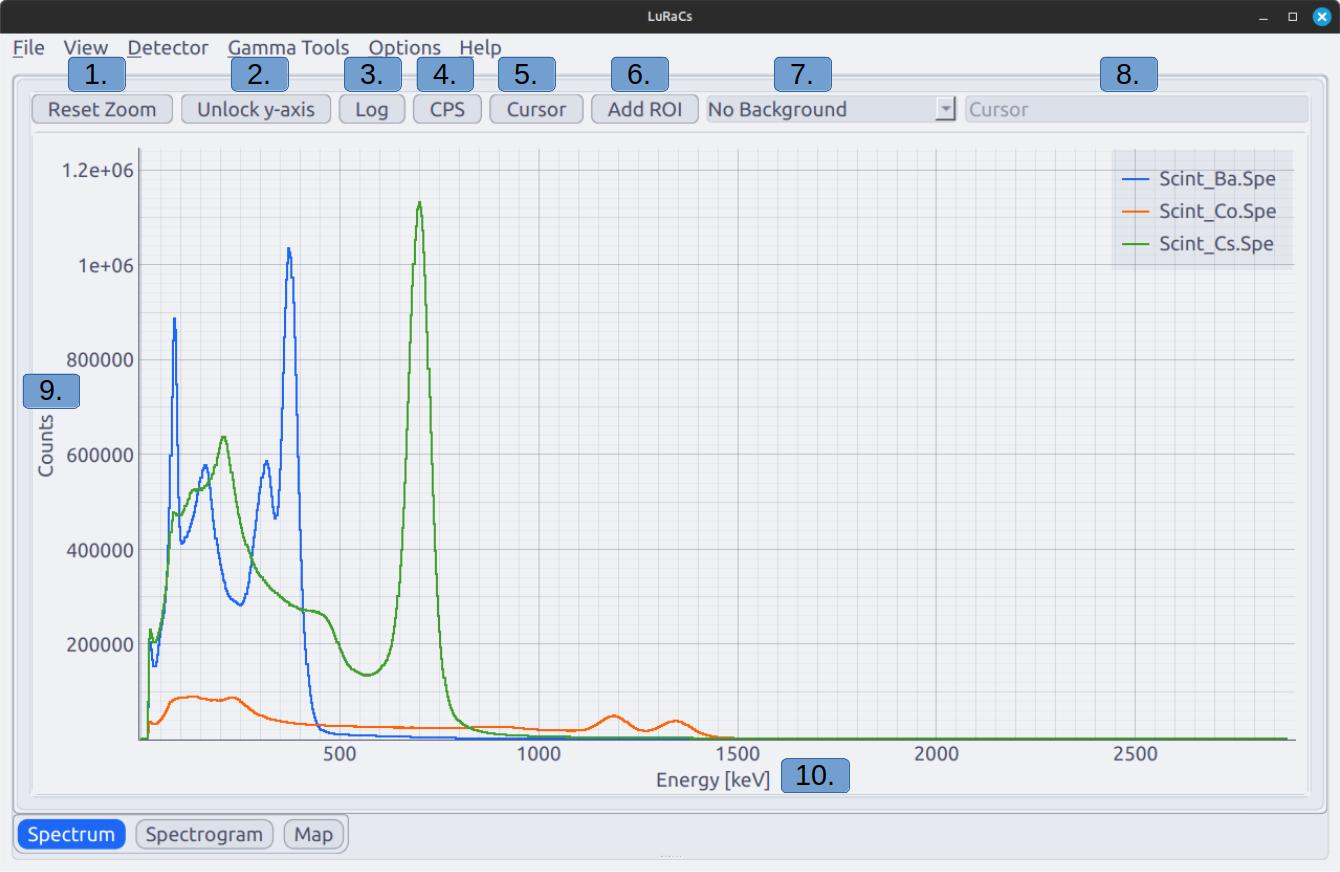
\includegraphics[width = .9\linewidth]{images/interface/spectrum_view.jpg}
    \caption{Spectra of Ba-133, C-60 and Cs-137 displayed in \textit{Combined Spectrum View}.}
    \label{fig:spectrum_view}
    \begin{flushleft}
        \begin{enumerate}
            \item \textbf{Rest Zoom} resets the zoom of the spectrum view and locks the y-axis if unlocked.
            \item \textbf{Unlock y-axis} allows the y-axis to be zoomed independently (by scrolling the wheel of the mouse) and disables autoscaling.
            \item \textbf{Log} set the scale of the y-axis to logarithmic or reset back to linear scale.
            \item \textbf{CPS} normalises the spectrum to the live time, or real time if live time is not available but real time is.
            \item \textbf{Cursor} toggles the spectrum cursor, see \autoref{fig:spectrum_with_cursor}.
            \item \textbf{Add ROI} adds a customisable \textit{region of interest} to the spectrum, see \autoref{fig:spectrum_with_roi}.
            \item Switch the use of background spectrum. Options are \textit{No background}, \textit{Background overlay} and \textit{background subtract}. See the section above.
            \item Display for info from the cursor, see \autoref{fig:spectrum_with_cursor}.
            \item The y-axis show either total counts or time normalised counts in units of \unit{\per\second}.
            \item The x-axis always display energy in units of keV.
        \end{enumerate}
    \end{flushleft}
\end{figure}

\textit{Regions of interest} (\textbf{ROI}) are sub regions of the spectrum bounded in energy and are useful in the analysis of spectrum peaks. Spectrum peaks can in most cases be approximated with a Gaussian function, knowing the function parameters is useful for many analyses. LuRaCs provides a method for fitting Gaussian functions to peaks inside ROIs and do so by default. These fits are required by other tools in the application. However, ROIs can also be configured to not perform fits. In these cases, only the total counts within each ROI are calculated.

\begin{figure}[H]
    \centering
    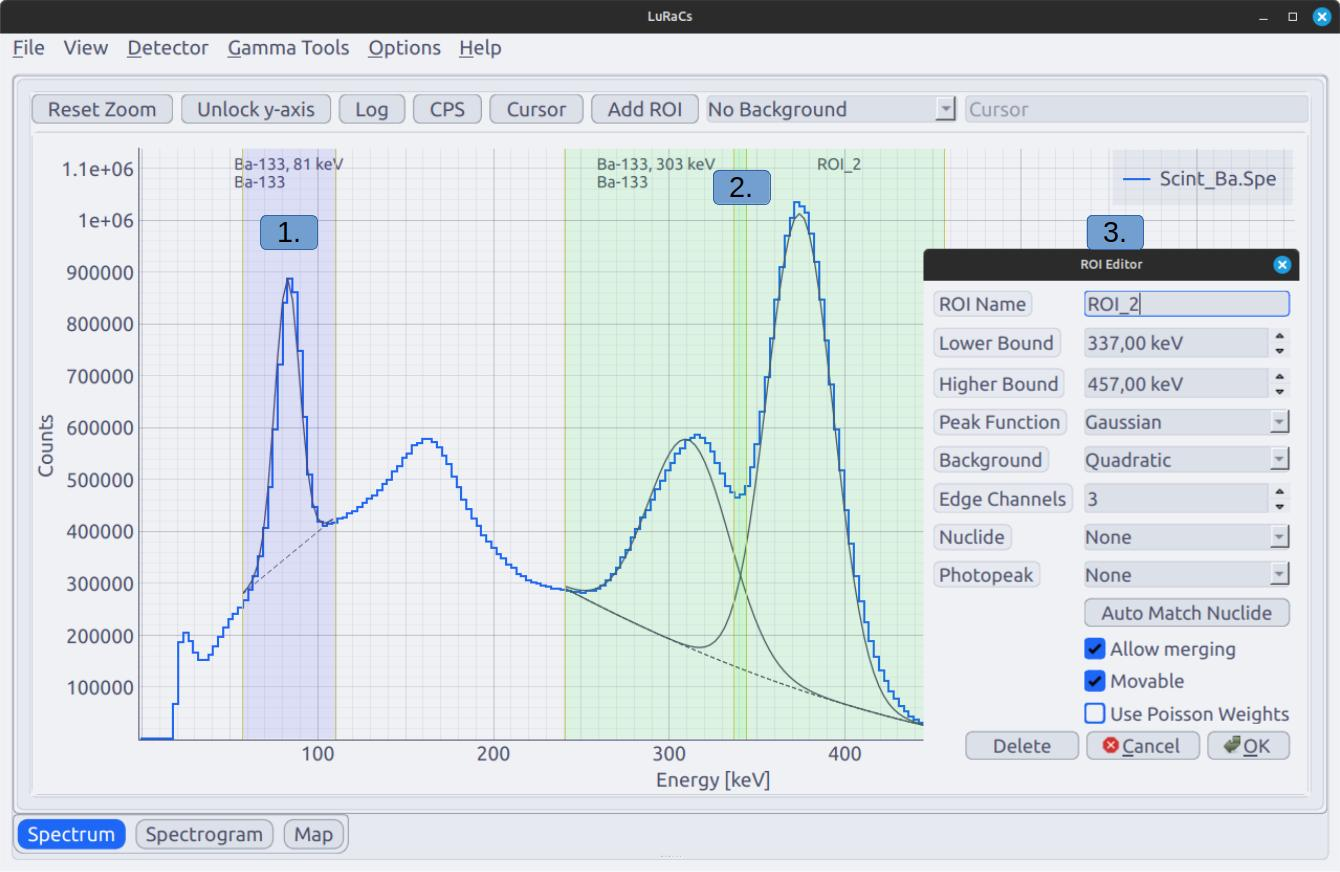
\includegraphics[width = .9\linewidth]{images/interface/spectrum_with_roi.jpg}
    \caption{A Ba-133 spectrum with three ROIs, two are merged and fitted to the same background. The ROI editor is open for the right most ROI (ROI\_2).}
    \label{fig:spectrum_with_roi}

    \begin{flushleft}
        \begin{enumerate}
            \item A ROI with one peak and a fitted Gaussian peak and linear background.
            \item Two merged ROIs that fit two Gaussian peaks on a shared quadratic background.
            \item The ROI editor for 'ROI\_2', see \autoref{tab:ROI_editor}.
        \end{enumerate}
    \end{flushleft}
\end{figure}

\begin{table}[H]
    \centering
    \caption{ROI Editor options}
    \label{tab:ROI_editor}
    \begin{tabular}{p{.3\textwidth}p{.7\textwidth}}
    \toprule
    \textbf{Field} & \textbf{Description} \\ \midrule
    ROI Name & An alias for the ROI used for display purposes and easier identification. \\
    Lower Bound & The lower energy bound of the ROI. \\
    Upper Bound & The upper energy bound of the ROI. \\
    Peak Function & The type of function fitted to the peak. Options are: \textit{Guassian}, \textit{None} \\
    Background & Type of function used as peak background. Options are: \textit{None}, \textit{Linear}, \textit{Quadratic} \\
    Edge Channels & The number of channels inside the ROI from the upper and lower bounds of the ROI used to fit the background. \\
    Nuclide & Assign a nuclide from the reference library to the ROI. Used for calculations by other tools. \\
    Photopeak & Choose the specific photon emission associated with the peak in the ROI. Options are based on the chosen nuclide. \\
    Auto Match Nuclide & Attempt to automatically find the nuclide and emission of the peak. If any nuclides are checked in the \textit{Isotopics}-tab, see section \ref{sec:isotopics}, the match is limited to these. Blind matches are often unreliable. \\
    Allow Merging & Allow the ROI to merge with other ROIs with merging allowed. \\
    Movable & If the ROI can be moved or its bounds adjusted by using the mouse. \\
    Use Poission Weights & Apply a 1/$\sigma$ weight to the optimisation to force the peak to emulate a Poission distribution. \\
    \bottomrule

    \end{tabular}
\end{table}

\begin{figure}[H]
    \centering
    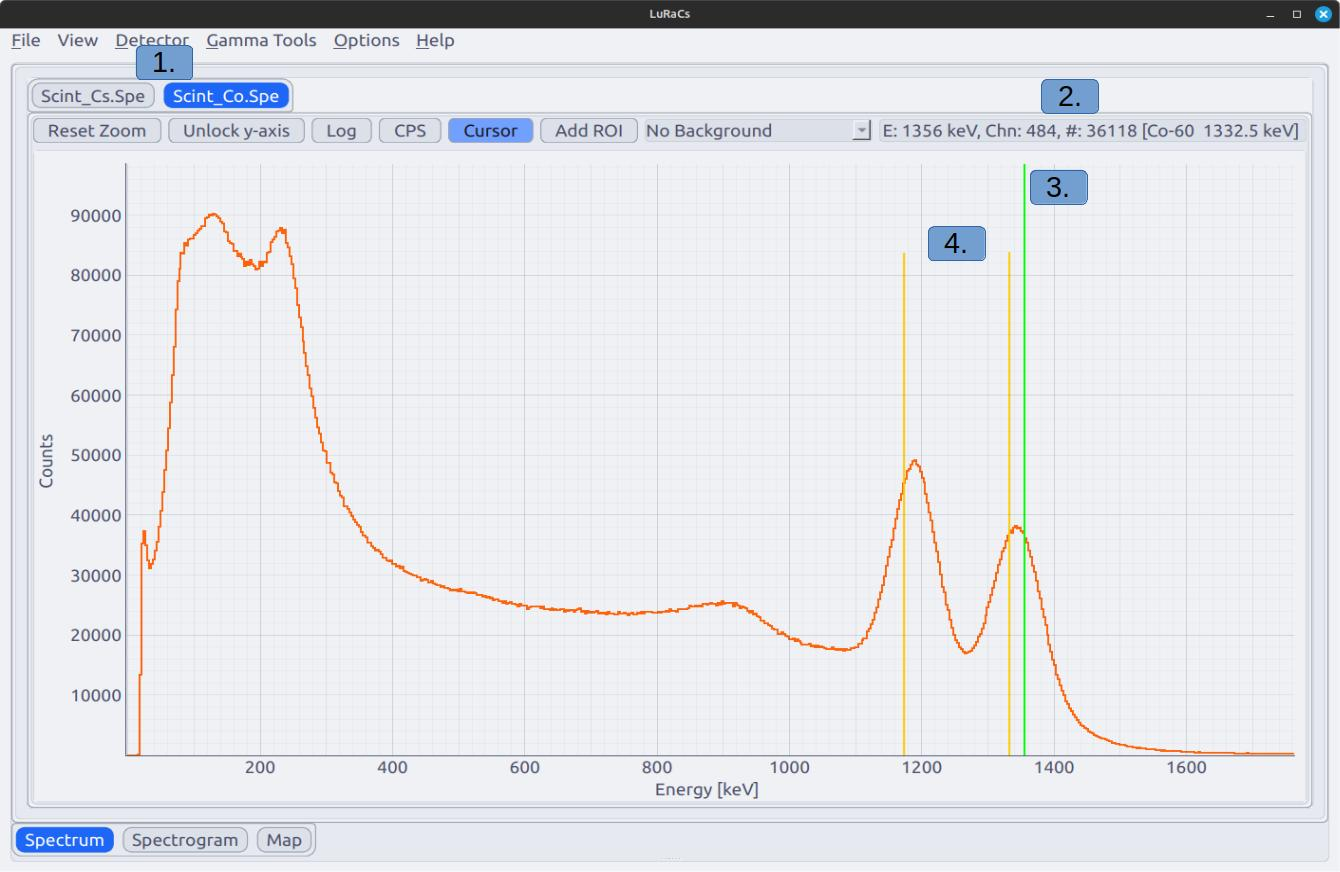
\includegraphics[width = .9\linewidth]{images/interface/spectrum_with_cursor.jpg}
    \caption{Co-60 spectrum with an active cursor.}
    \label{fig:spectrum_with_cursor}

    \begin{flushleft}
        \begin{enumerate}
            \item Tabs for selecting spectrum in \textit{Tabbed Spectrum View}.
            \item Spectrum information at the position of the cursor, showing of the corresponding energy and channels number, the number of counts in the channel, closest reference emission line as [\textit{nuclide} \textit{Emission Energy} \textit{Decay chain if applicable}]. Channel and channel counts are only displayed in tabbed spectrum view.
            \item Cursor in the spectrum.
            \item These always appear for the emission closest to the cursor in energy and does not weigh intensity or anything else. This can be disabled by \texttt{View -> Spectrum -> Show Cursor Emissions}.
        \end{enumerate}
    \end{flushleft}
\end{figure}
\subsubsection{Spectrogram}
A spectrogram allows acquisition of data time-series. A spectrogram stores data with specified time intervals and can be displayed in a waterfall plot. It is also the function LuRaCs utilise for mobile measurements. If a GPS is connected, the geolocation data is automatically stored in the spectrogram. These measurements can be visualised on the embedded Map (or an online map).

\begin{figure}[H]
    \centering
    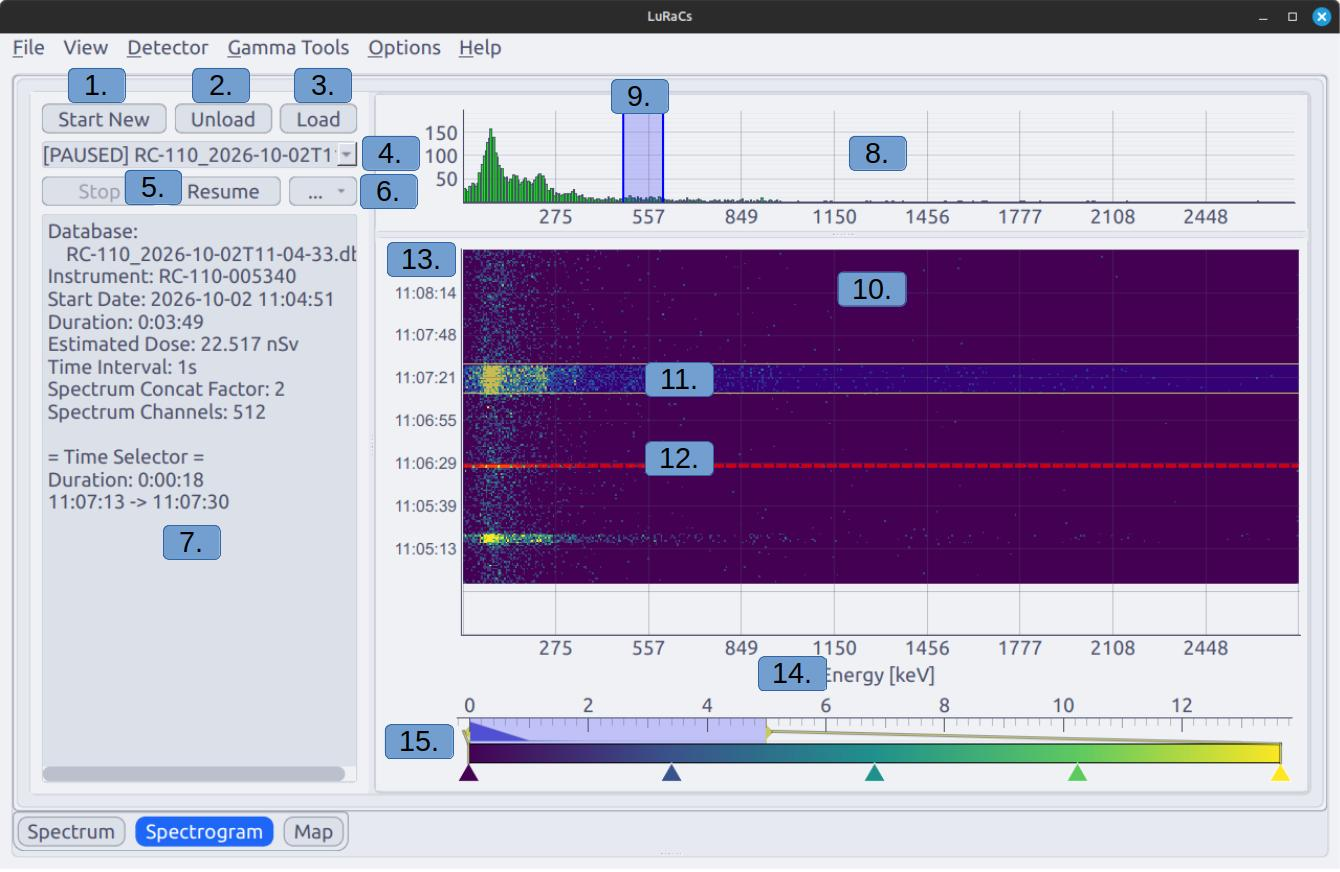
\includegraphics[width = .9\linewidth]{images/interface/spectrogram_view.jpg}
    \caption{Acquisition of a spectrogram with the \textit{Time Selector} active and one ROI.}
    \label{fig:spectrogram_view}

    \begin{flushleft}
        \begin{enumerate}
            \item Opens a dialog for starting a new spectrogram.
            \item Close the viewed spectrogram.
            \item Shortcut to the Data Library Spectrogram page, see section \ref{sec:data_store}.
            \item Toggle the currently loaded spectrograms. Status is shown to the left as [ACTIVE], [LOADED] or [PAUSED].
            \item Pause or Resume data collection, requires that the same detector used to collect the previous data is connected.
            \item Options menu, see \autoref{fig:spectrogram_options}
            \item Current information stored in the spectrogram and information about the \textit{Time Selector}, if active.
            \item Count histogram. Shows either total accumulated spectrum when loading a previously acquired spectrogram, summed channel counts inside the \textit{Time Selector}, if active, or counts in the latest row.
            \item ROI illustrated in the histogram, can be removed with Mouse-2.
            \item Waterfall diagram of the spectrogram.
            \item \textit{Time Selector} to study the summed spectra within a specific time interval. Can be toggled in the options menu (6.).
            \item Data break line, illustrates that the time between measured points exceeds the Time Interval. Can indicate a lost connection and thus caution should be taken to verify data integrity. Can be toggled in the options menu (6.).
            \item Y-axis displays the timestamps of when each row was measured.
            \item X-axis display spectrum energy, if calibrated.
            \item Color slider for the waterfall diagram. The color map can be changed by clicking Mouse-2 on the gradient bar.
        \end{enumerate}
    \end{flushleft}
\end{figure}

The spectrogram format is based around an SQLite database, see section \ref{sec:file_spectrogram} for further details on the format. The following data is stored for each time point in the spectrogram:

\begin{itemize}
    \item Timestamp.
    \item Average count rate measured since the last time point.
    \item Average dose rate measured since the last time point.
    \item Device temperature at the time the data is stored.
    \item Longitude at the time the data is stored, if a GPS is available.
    \item Latitude at the time the data is stored, if a GPS is available.
    \item Spectrum difference since the previous data point was stored, as compressed binary.
    \item Meta data, stored as a utf-8 encoded and zlib compressed json-string. Examples of stored metadata include extended GPS data.
\end{itemize}

\paragraph{Exporting a spectrogram} is done trough the Data Library, accessed via the \textit{Load}-button (2.).

\begin{figure}[H]
    \centering
    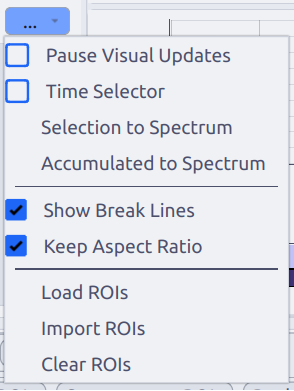
\includegraphics[width = .4\linewidth]{images/interface/spectrogram_options.png}
    \caption{Dropdown options menu in spectrogram pane, see \autoref{tab:spectrogram_options}.}
    \label{fig:spectrogram_options}
\end{figure}

\begin{table}[H]
    \centering
    \caption{Description of the possible operations in the spectrogram options menu}
    \label{tab:spectrogram_options}
    \begin{tabular}{p{.3\textwidth}p{.64\textwidth}}
    \toprule
    \textbf{Field} & \textbf{Description} \\ \midrule
    Pause Visual Updates & Stop the view spectrogram from updating while the measurement is still on going in the background. \textbf{This does not stop the recording of the spectrogram}. \\
    Time Selector & Add a selected ROI in the spectrogram (11.) that can indicate the specific time interval, as opposed to all other ROIs that have energy bounds, and show the sum over time of the channels in the top count histogram (8.). \\
    Selection to Spectrum & Export the data within a selected time interval to the Data Library as a spectrum. \\
    Accumulated to Spectrum & Export the accumulated counts to the Data Library as a spectrum. \\
    Show Break Lines & If the red lines (12.) indicating if the interval between two rows exceed the specified save interval should be shown. \\
    Keep Aspect Ratio & If the pixels in the spectrogram should always be square. For detectors with many channels it can be useful to turn this off. If this option is off the pixels in the spectrogram may not align with the corresponding bar in the count histogram. \\
    Load ROIs & Shortcut to the ROI tab of the Data Library. \\
    Import ROIs & Load ROIs from a LuRaCs XML-file. \\
    Clear ROIs & Remove all spectrogram ROIs \\
    \bottomrule
    \end{tabular}
\end{table}
\subsubsection{Map}
Loading a map enables viewing of geographic measurements made with a spectrogram and a GPS. Maps can be loaded from online API requiring an internet connection or loaded from a \textit{.pmtiles}-file for offline use. Compatible APIs and files are offered by several sources, the software \textit{QGis} offers support for exporting \textit{.pmtiles} from other formats using plugins.

\paragraph{Disclaimer} LuRaCs does not provide or distribute any map data. Users are responsible for ensuring that such data or tile services they use with LuRaCs are obtained and used in accordance with the applicable licenses, terms, and usage restrictions.

The map is rendered using Qt's web engine, making it a powerful but resource demanding tool. Using offline maps can require a lot of system memory since the server needs to cache tiles for a smooth view. It is therefore recommended to use a system with enough memory when this option is applied. However, both the map and datapoints are rendered using GPU acceleration with WebGL, allowing for 10 000s of points to be displayed without excessive stress on the system. For reference, a Raspberry Pi 5 with 8 GB of RAM can render a 1.4 GB map file without any stutter, total memory usage was approximately 2 GB.

\begin{figure}[H]
    \centering
    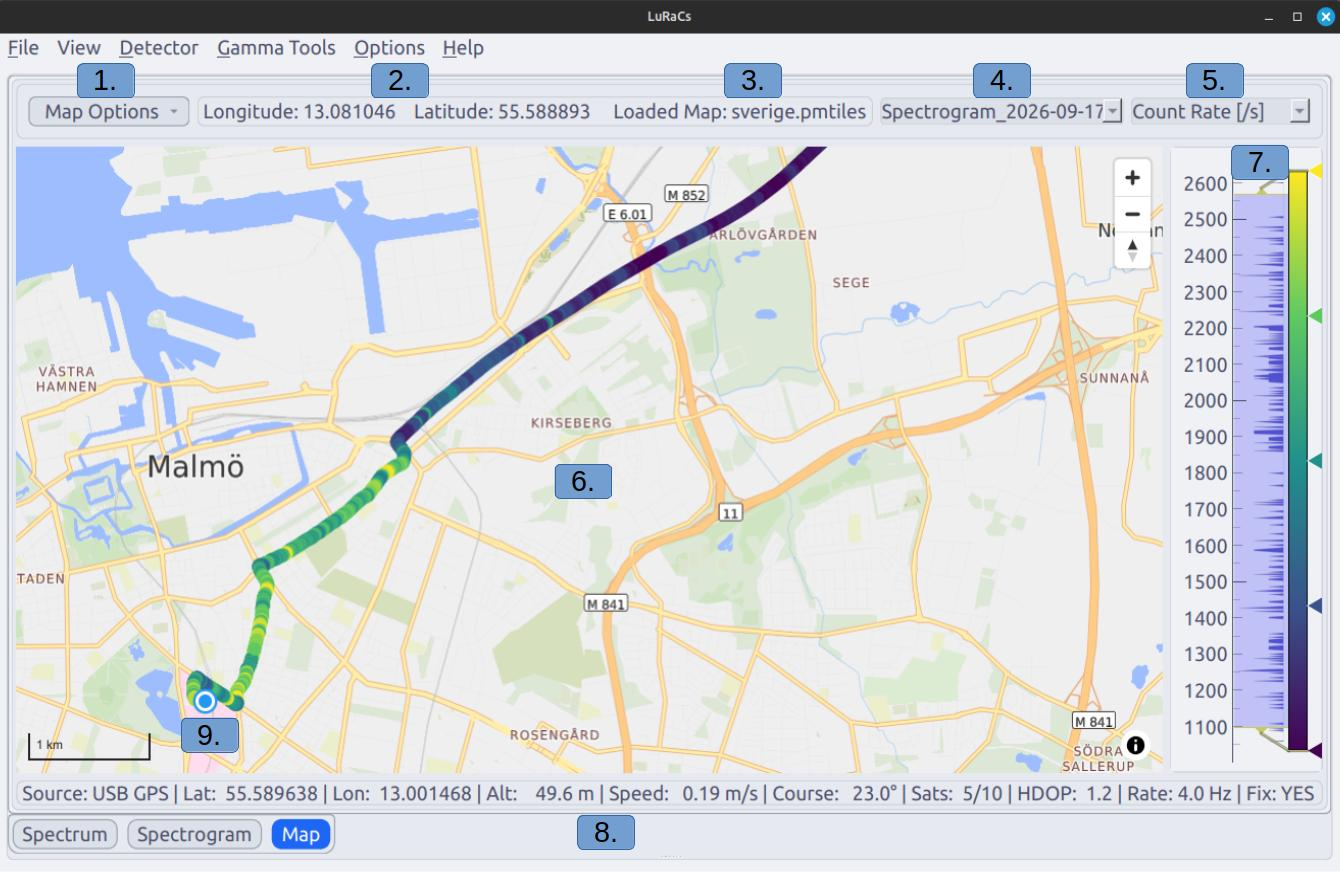
\includegraphics[width = .9\linewidth]{images/interface/map_view.jpg}
    \caption{Map with a loaded track and a connected GPS.}
    \label{fig:map_view}
    \begin{flushleft}
        \begin{enumerate}
            \item Options menu for loading maps, importing and exporting simple tracks.
            \item Longitude and Latitude for the position of the cursor.
            \item Name of the loaded map.
            \item List of loaded spectrograms. If the selected spectrogram does not contain any geolocation data, no measurement points are displayed.
            \item Selector for what data is shown: total count rate, dose rate or count rate inside a loaded ROI.
            \item Main map view.
            \item Selector for color gradient, used for the track points and a histogram over the measured values. The color map can be changed by clicking Mouse-2 on the gradient bar.
            \item Live data from the GPS.
            \item Current GPS position, always displayed as a white and blue circle.
        \end{enumerate}
    \end{flushleft}
\end{figure}

\paragraph{Load a map} is done from \texttt{Map Options -> Load Online/Offline Map}. An offline map takes the form of a \textit{.pmltiles} file. By choosing this option prompts the selection of such a file. Choosing to load an online map prompts the user to enter a URL, to a tile serving API, possibly including an API key. The checkbox allows for saving the most recently used URL. If a personal API key is used, be aware that URLs are saved unencrypted.
\subsubsection{Measure}\label{sec:measure_view}
The measure tab allows for making controlled measurements with a simplified interface. These measurement can then be exported as clean, human readable reports while still being valid spectrum files. The interface is designed to be intuitive and this tab serves as the only interface for LuRaCs-Si, as described in the introduction. Buttons will indicate the order they should be pressed and the only submenus required are to connect detectors and to export the report. 

\begin{figure}[H]
    \centering
    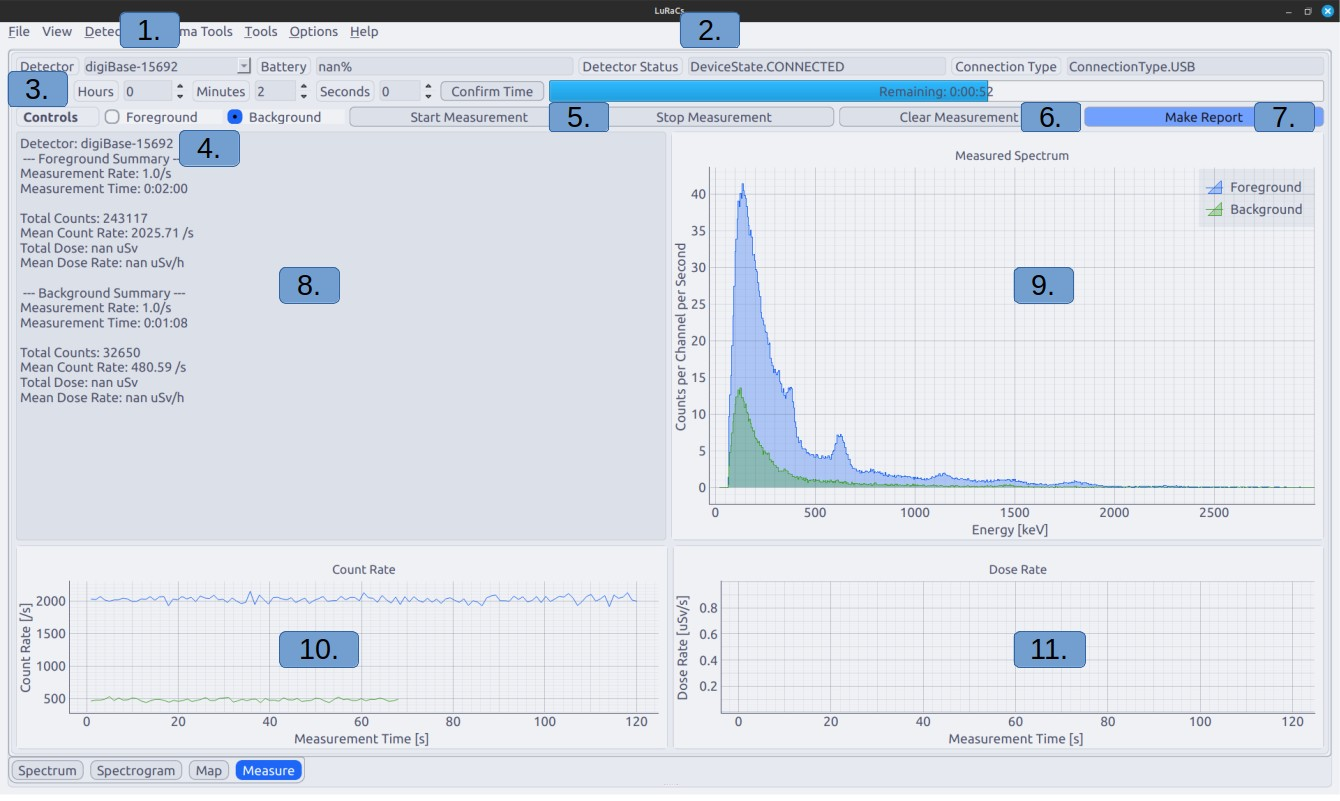
\includegraphics[width = .9\linewidth]{images/interface/measure_view.jpg}
    \caption{The measure view with an on going measurement using a 3"x3" NaI detector. The foreground spectrum is of an antique containing Ra-226 and the background is a regular office. The detector does not have a battery and does not output dose data, therefore these reading are \texttt{nan}.}
    \label{fig:measure_view}
    \begin{flushleft}
        \begin{enumerate}
            \item Selected detector. If the detector is changed all measurements are reset to avoid mixing measurements for different detectors. This is preceded by a question dialog so results are not lost by accident.
            \item Detector status bars, shows the same data as in the \textit{Detectors}-tab, see section \ref{sec:detectors}
            \item The measurement timer to determine the length of a measurement. The duration is set in the spinboxes and must be applied with \texttt{Confirm Time}, which while be marked upon changing a time value. The bar shows remaining time. The same time can be used for fore- and background without applying it again.
            \item Selects if the measurement is the fore- or background.
            \item \texttt{Start Measurement} and \texttt{Stop Measurement} do what they say. Each time an ongoing measurement is stopped the timestamp is logged and included in the report.
            \item Clears the measurement selected in (4.).
            \item Opens the Report Dialog for creating a report form the measurement, see \autoref{fig:report_form}.
            \item Main information window that displays summary information about the measurements.
            \item Count histogram of the fore- and background. Pulls the energy calibration form the spectrum in the \textit{Spectrum}-tab.
            \item Count Rate graph.
            \item Dose Rate graph, always in \unit{\micro\sievert\per\hour}
        \end{enumerate}
    \end{flushleft}
\end{figure}

\begin{figure}[H]
    \centering
    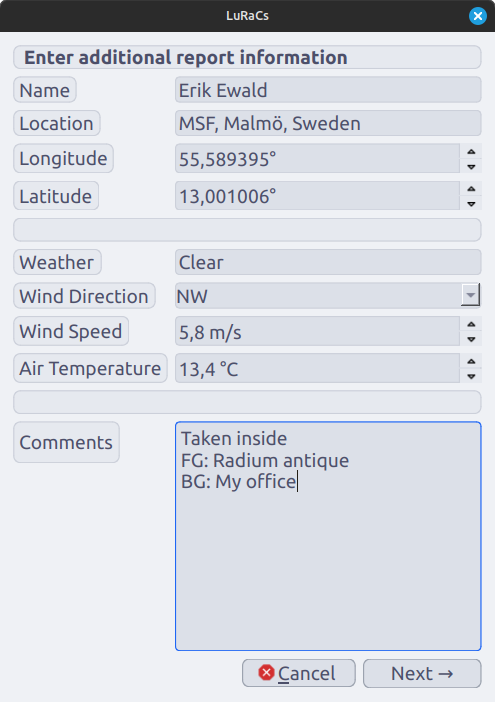
\includegraphics[width = .4\linewidth]{images/interface/report_form.png}
    \caption{Report Form opened by pressing (7.) in \autoref{fig:measure_view}.}
    \label{fig:report_form}
\end{figure}
\subsection{Secondary Tabs}

\subsubsection{Spectrum Info}
Displays information about loaded spectra, both from files (which ones, write out) and detectors memory.
\begin{figure}[H]
    \centering
    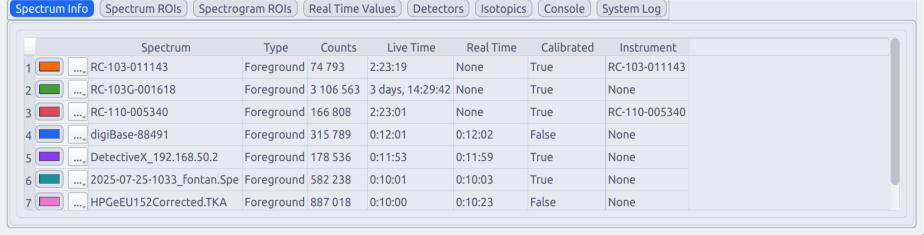
\includegraphics[width = .9\linewidth]{images/interface/spectrum_tab.jpg}
    \caption{Spectrum Info Tab. For imported spectra with other formats than \texttt{XML} or \texttt{N42} file extensions are kept in the name.}
    \label{fig:spectrum_info}
\end{figure}

\begin{table}[H]
    \centering
    \caption{Description of the columns in the Spectrum Info tab}
    \label{tab:spectrum_info_table}
    \begin{tabular}{p{.3\textwidth}p{.64\textwidth}}
    \toprule
    \textbf{Column} & \textbf{Description} \\ \midrule
        Column 0 & Color button allowing for changing the color of the displayed. Options button marked with '...', see \autoref{tab:spectrum_info_options_menu}. \\
        Spectrum & The name of the spectrum or connected detector. A spectrum retrieved from a detector is automatically given the same name as the detector, this can not be changed unless the spectrum is saved or exported. \\
        Type & \textit{Foreground} or \textit{Background}, these share the same name in the 'Spectrum'-column for the same spectrum. This division exists because a spectrum can contain both foreground and background that have different measurement times and total counts. \\
        Live Time & The live time (h:min:s) of the measurement, accounting for dead time. \\
        Real Time & The real time (h:min:s) of the measurement. \\
        Calibrated & \textit{True} or \textit{False}, if an energy calibration is detected and applied. \\
        Instrument & Which instrument is assigned to the spectrum, see section \ref{sec:definitions} \\
    \bottomrule
    \end{tabular}
\end{table}

\begin{table}[H]
    \centering
    \caption{Description of the options menu opened by the button marked '...' on each row. The type 'Background's are limited to only the 'Remove' option.}
    \label{tab:spectrum_info_options_menu}
    \begin{tabular}{p{.3\textwidth}p{.64\textwidth}}
    \toprule
    \textbf{Field} & \textbf{Description} \\ \midrule
        Save & Save the spectrum to the Data Library. \\
        Export & Export the spectrum to a standalone file in the following formats: \texttt{XML}, \texttt{CSV}, \texttt{xlsx}. \\
        Hide/Show & Toggle visibility of the spectrum in the spectrum view. ROIs are not applied to hidden spectra. \\
        Edit & Edit properties of the spectrum, see \autoref{}. \\
        Remove Spectrum & Remove the spectrum and disconnect a detector associated with the spectrum.
    \\ \bottomrule
    \end{tabular}
\end{table}
\subsubsection{Spectrum ROIs}

\begin{figure}[H]
    \centering
    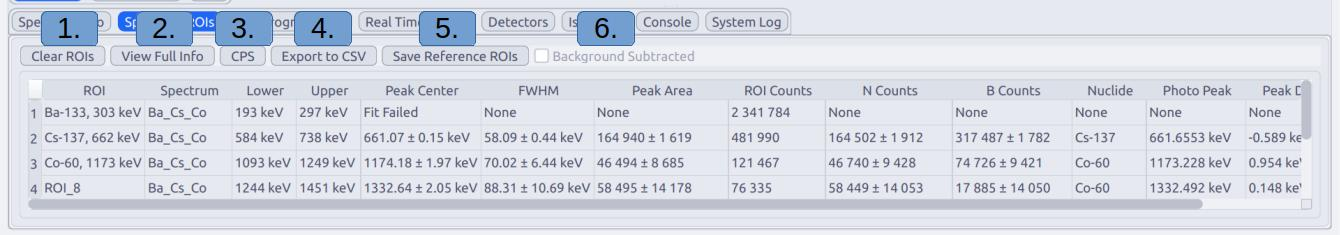
\includegraphics[width = .9\linewidth]{images/interface/spectrum_roi_info_tab.jpg}
    \caption{Spectrum ROIs tab}
    \label{fig:spectrum_rois}
    \begin{flushleft}
        \begin{enumerate}
            \item Remove all loaded ROIs from all spectra.
            \item Debug view of all data contained in the loaded ROIs.
            \item Apply time normalisation to the ROI data.
            \item Export the acquired and calculated data, including live time, of each ROI to a CSV-file.
            \item Save ROI references to the Data Library, see section \ref{sec:data_store}, for later access. These ROI references save the settings of the ROI (bounds, emission, name, fit type, etc.) but not the ROI data.
            \item Icon to display if the spectrum is background subtracted. Background subtraction effects the results of the ROI calculations.
        \end{enumerate}
    \end{flushleft}
\end{figure}
\subsubsection{Spectrogram ROIs}
Spectrum ROIs apply a curve fitting whereas Spectrogram ROIs do not. When applying a ROI to a spectrogram it sums the counts from all the channels within its bounds and do so for every row in the spectrogram. The results are displayed in count rate, as the number of counts are normalised to the save interval. This makes it easier to compare spectrograms recorded with different save intervals.

\begin{figure}[H]
    \centering
    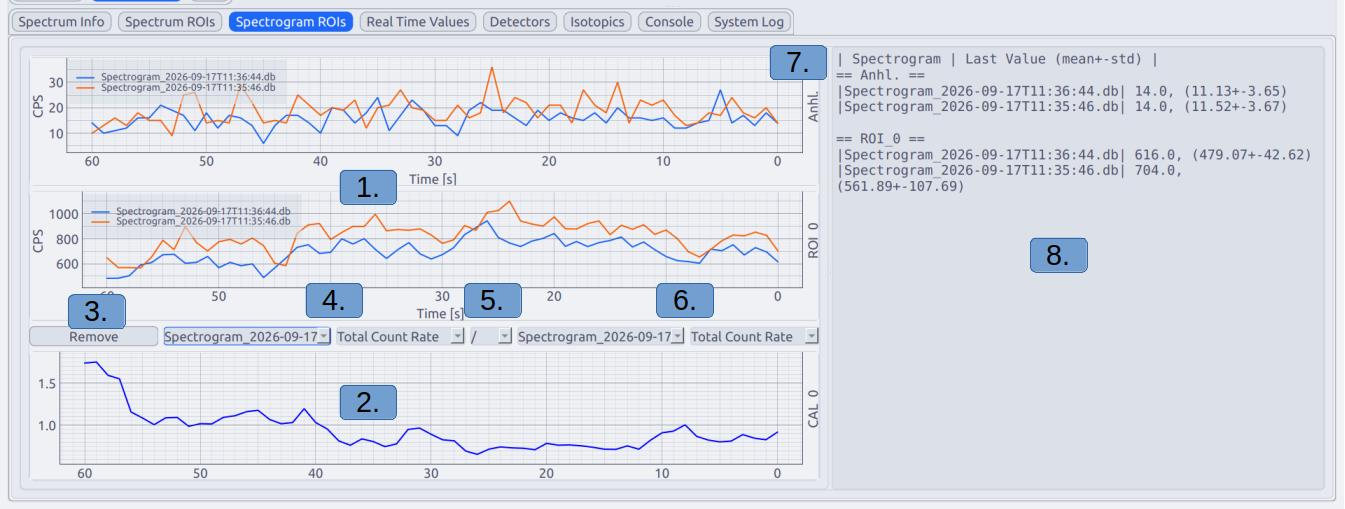
\includegraphics[width = .9\linewidth]{images/interface/spectrogram_rois.jpg}
    \caption{Spectrogram ROI tab showing two loaded spectrograms with two loaded ROIs. A \textit{Calculation ROI} is also added.}
    \label{fig:spectrogram_rois}
    \begin{flushleft}
        \begin{enumerate}
            \item Plots of two spectrogram ROIs evaluated on two separate spectrograms.
            \item Calculation ROI
            \item Button for removing the calculation ROI
            \item Settings for the first spectrogram in the calculation ROI. The first combobox lists loaded spectrograms and the second selects the data, total count rate or count rate from a ROI.
            \item Mathematical operations for comparing the ROI values are: \texttt{+}, \texttt{-} or \texttt{/}.
            \item Settings for the second spectrogram in the calculation ROI. These setting are the same as for the first (4.).
            \item ROI names. Calculation ROIs currently only have a tag containing a serial number on the form \texttt{CAL\_X}. Currently, they can not be renamed.
            \item ROI data in text form. Shown is the latest value and (mean+-std) calculated from the data shown in the plot.
        \end{enumerate}
    \end{flushleft}

\end{figure}

During mobile measurements LuRaCs offers the selection to monitor several ROIs simultaneously. For this e a 'Compact View' can be used. This is enabled under \texttt{View -> Spectrogram ROis -> Compact View}. This function strips all GUI elements from the plots, except the y-ticks and the plot itself.

\begin{figure}[H]
    \centering
    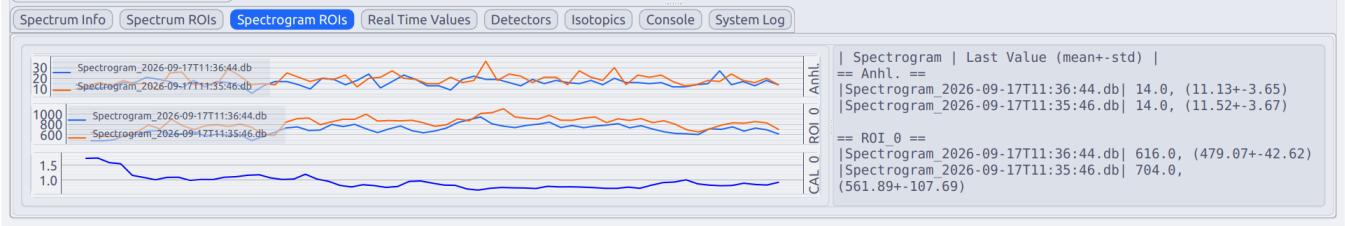
\includegraphics[width = .9\linewidth]{images/interface/spectrogram_rois_compact.jpg}
    \caption{Same spectrograms and ROIs as in \autoref{fig:spectrogram_rois} but in compact view.}
    \label{fig:spectrogram_rois_compact}
    
\end{figure}

\textit{Calculation ROIs} are plots calculated from the results of other ROIs. \textbf{These perform element wise operations and do not account for differences in measurement parameters}. Element 0 from ROI 0 is combined with Element 0 of ROI 1, regardless of measurement date or spectrogram save interval.
\subsubsection{Detectors}\label{sec:detectors}
Information and status of connected detectors are displayed in this tab.
\begin{figure}[H]
    \centering
    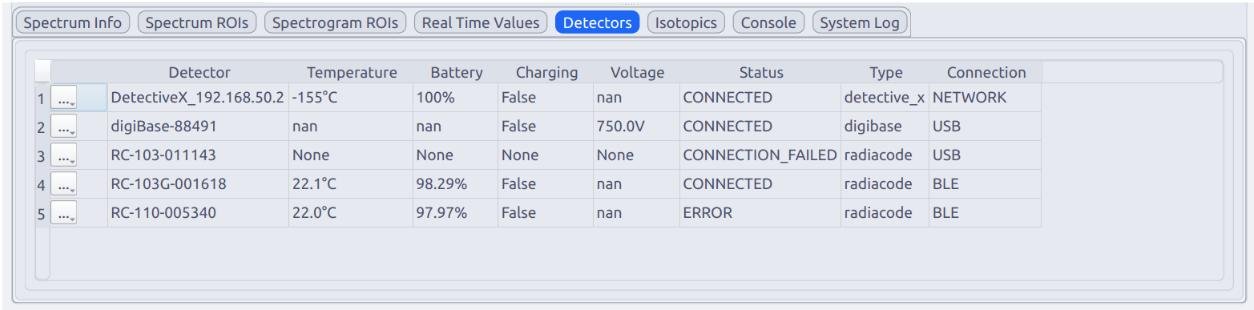
\includegraphics[width = .9\linewidth]{images/interface/detectors_tab.jpg}
    \caption{List of connected detectors. An entry can not be removed, if a detector is disconnected it is listed as \texttt{STOPPED}.}
    \label{fig:detector_tab}
\end{figure}

\begin{table}[H]
    \centering
    \caption{Description of the columns in the Detectors tab}
    \label{tab:detectors_tab}
    \begin{tabular}{p{.3\textwidth}p{.64\textwidth}}
    \toprule
    \textbf{Column} & \textbf{Description} \\ \midrule
        Column 0 & Options button marked with '...', see \autoref{tab:detectors_options_button}. \\
        Detector & The name of the detector. \\
        Temperature & The temperature reading from the detector in $^\circ$C. Most detectors report the ambient temperature but some, like the Detective X, report the cooled crystal temperature, as seen in \autoref{fig:detector_tab}. \\
        Battery & The current battery level in \%. \\
        Charging & Indicate if the detector is connected to a power source. \\
        Voltage & The actual voltage reported of the detector in V. \\
        Status & Detector state reported as one of the following options: 
        \begin{itemize}
            \item \texttt{UNINITIALIZED} - Detector client created but not started.
            \item \texttt{CONNECTING} - The detector is starting.
            \item \texttt{CONNECTED} - The detector is connected and running. Default for normal detector function.
            \item \texttt{CONNECTION\_FAILED} - Detector start failed. Check System Log.
            \item \texttt{CONNECTION\_LOST} - Connection was lost after a successful start. Not universally implemented.
            \item \texttt{STOPPING} - The detector has received and acknowledged the command to stop.
            \item \texttt{STOPPED} - The detector has successfully stopped.
            \item \texttt{ERROR} - An error occurred while connected and the detector is no longer functioning as expected.
        \end{itemize} \\
        Type & Type of detector by the name defined in the detector client. \\
        Connection & How the detector is connected. Can be \texttt{BLE, USB} or \texttt{NETWORK}. \\
    \bottomrule
    \end{tabular}
\end{table}

\begin{table}[H]
    \centering
    \caption{Description of the options menu in the detector tab, opened with the button marked '...' in the table.}
    \label{tab:detectors_options_button}
    \begin{tabular}{p{.3\textwidth}p{.64\textwidth}}
    \toprule
    \textbf{Field} & \textbf{Description} \\ \midrule
        Disconnect & Sends a stop signal to the detector. \\
        Reset Spectrum & Signals to the selected detector to clear its spectrum. \\
        Start Acquisition & Signals to the selected detector to start spectrum acquisition. \\
        Stop Acquisition & Signals to the selected detector to stop spectrum acquisition. \\
        Make Instrument & Shortcut for creating a \textit{Unique Instrument} for the detector based on a \texttt{Generic Instrument} and save the current calibration of the connected spectrum. Useful for detectors that do not Library their own energy calibration. \\
        Settings & Opens the detector settings dialog, see \autoref{fig:detector_settings_calibration} and \autoref{fig:detector_settings_mca}. \\
    \bottomrule
    \end{tabular}
\end{table}

\begin{figure}[H]
    \centering
    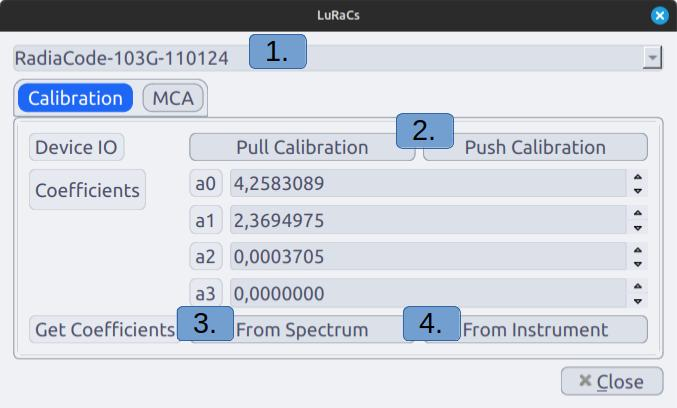
\includegraphics[width = .6\linewidth]{images/interface/detector_settings_calibration.jpg}
    \caption{Detector settings dialog showing the options for setting device calibration.}
    \label{fig:detector_settings_calibration}
    \begin{flushleft}
        \begin{enumerate}
            \item Unique Instrument from the library to pull settings from.
            \item Interact with the detector. \texttt{Pull Calibration} will request a calibration from the detector set in the coefficients buffer, not possible for all detectors. \texttt{Push Calibration} will attempt to set the calibration of the detector, not possible for all detectors.
            \item Pull the calibration coefficients from the spectrum connected to the detector and set in the coefficients buffer.
            \item Pull the calibration coefficients from the instrument set in (1.) and set in the coefficients buffer
        \end{enumerate}
    \end{flushleft}
\end{figure}

\begin{figure}[H]
    \centering
    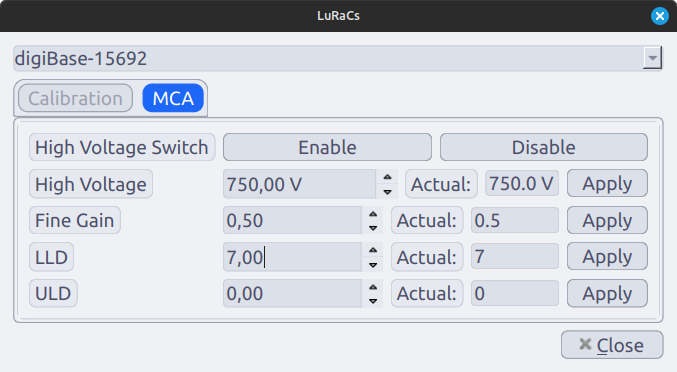
\includegraphics[width = .6\linewidth]{images/interface/detector_settings_mca.png}
    \caption{Detector settings dialog showing the options for MCA settings. The first column of spinboxes show the requested setting and the second row shows the actual value reported by the instrument. \texttt{Apply} attempts to set the given value to the detector.}
    \label{fig:detector_settings_mca}
    \begin{tabular}{ll}
    LLD & Lower Level Discriminator \\
    ULD & Upper Lever Discriminator
    \end{tabular}
  
\end{figure}
\subsubsection{Isotopics}\label{sec:isotopics}
LuRaCs provides a library of data for a selection of common radionuclides that can be accessed under the tab Isotopics. This datacan be used to draw reference lines for emissions in the spectrum plot. Most of the nuclide data is sourced from \textit{Laboratoire National Henri Becquerel}, the others from sources elsewhere. A citation is provided for each nuclide whereas full references can be found under \texttt{Help -> Bibliography}.

\begin{figure}[H]
    \centering
    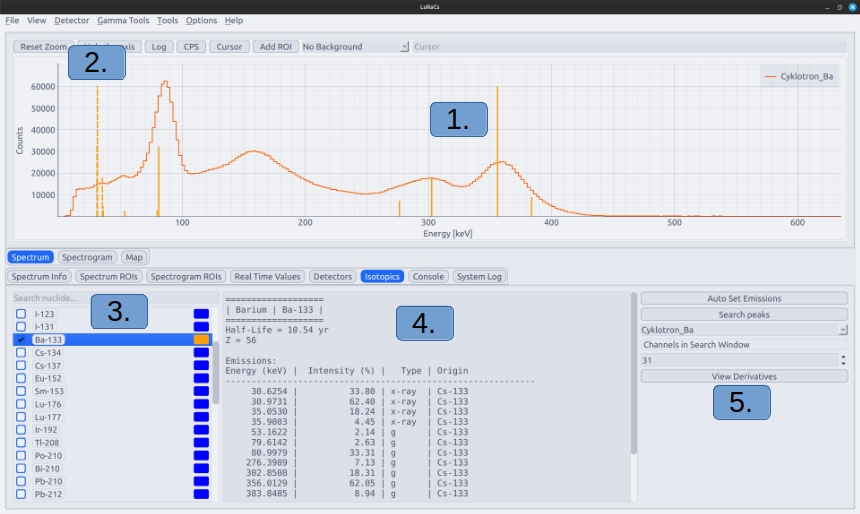
\includegraphics[width = .9\linewidth]{images/interface/isotopics.jpg}
    \caption{Ba-133 spectrum with Ba-133 selected in the Isotopics Tab.}
    \label{fig:isotopics}
    \begin{flushleft}
        \begin{enumerate}
            \item Spectrum and gamma emission lines, drawn as solid lines. Line height corresponds to emission intensity,
            \item X-ray emission lines, drawn as dashed lines. Line height corresponds to emission intensity.
            \item Nuclide list, select nuclide with the checkbox to the left and change colour of the gamma emission lines with the right coloured button.
            \item Information of the current marked nuclide.
            \item Peak automation, see bellow.
        \end{enumerate}
    \end{flushleft}
\end{figure}

Auto matching nuclides to ROIs is accomplished by using the centroid of a fitted peak and finding emission close in energy. The matching is weighted by the emission intensity so a strong emission will be chosen over a weak if they are the same distance from the peak centroid. By selecting nuclides the auto matching of nuclides to ROIs, including from using the button inside the \textit{ROI Editor}, are limited emission from the selected nuclides. Using auto match nuclides against all possible candidates are often unreliable, especially if the energy calibration is imperfect. 

The peak search is based on Savitzky-Golay smoothing and the filter derivatives to compute peak candidates. The computed candidates are filtered, the accepted peaks are then added as ROIs. The length of the window in the Savitzky-Golay filter can be set in units of channels. 
\subsubsection{Console}
The console allows for entering text commands to control the application and running scripts for simple automation. See \autoref{subsec:cli} for information on available commands and their usage.

The Console can be used for light automation by using the \texttt{exec} command and providing a file path. The file is executed line by line and can used to quickly start set up a measurement session.
\subsubsection{System Log}
The System Log displays messages from the application and detector clients. If something crashes the error and traceback will be displayed here.
\subsection{Gamma Tools}
\subsubsection{Calibration}
Calibration is the operation of setting the energy each channel corresponds to.

\begin{figure}[H]
    \centering
    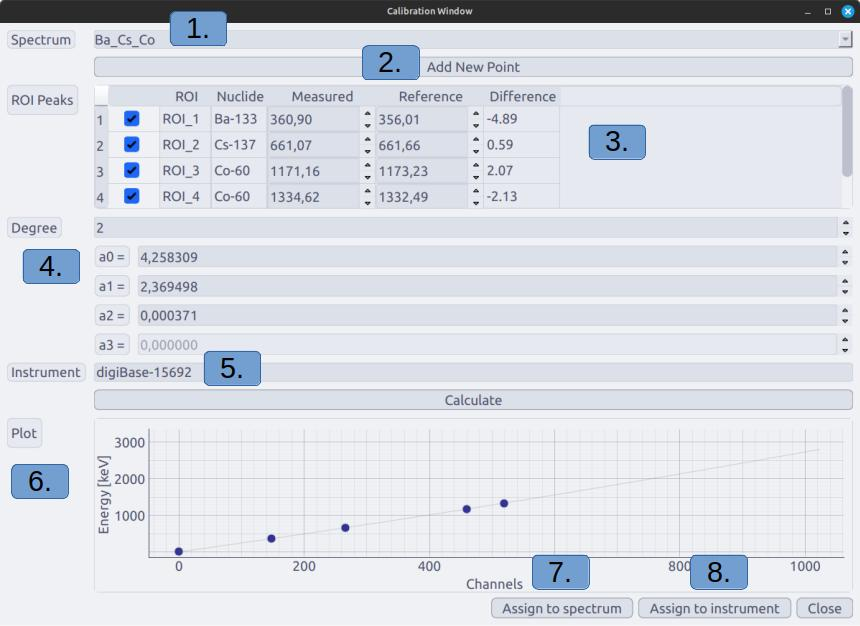
\includegraphics[width = .7\linewidth]{images/interface/gtools_calibration.jpg}
    \caption{Calibration window of a spectrum with 4 ROIs and assigned nuclides.}
    \label{fig:gtools_calibration}
    \begin{flushleft}
        \begin{enumerate}
            \item Which spectrum should be used for the calibration. For each calibration, data from only one spectrum is allowed.
            \item Add a calibration point, that is not associated with a ROI. Measured and Reference energies must be set manually.
            \item Current calibration points detected and their corresponding information. When unchecking a row it will be ignored in the calculation.
            \item Polynomial degree of the calibration function and the current coefficients. Coefficients can be changed manually but will be updated by pressing \texttt{Calculate}.
            \item The instrument used for acquiring the spectrum. This is fixed and can not be changed here, instead edit the spectrum before starting the calibration, see section \ref{}.
            \item Plot showing the energy as a function of channels based on the latest calculated coefficients.
            \item Assign the coefficients to the \textit{Unique Instrument} shown in (5.).
            \item Assign the new calibration coefficients and recalculate the x-axis for the spectrum selected in (1.), updating the view in the Spectrum-tab. Note, this will not change the calibration of an already started spectrogram.
        \end{enumerate}
    \end{flushleft}
\end{figure}
\subsubsection{Deconvolution}
This tool does more than simply reducing the effect of energy resolution but will still be referred to as a deconvolution operation. Deconvolution in this sense is more similar to reconstruction as in image reconstruction in nuclear medicine, it employs the ML-EM algorithm. By using a detector response matrix, most simply acquired using Monte Carlo-simulations, the effects of the detector resolution, scattering in the detector and other effects can be reduced. The response matrix represents the expected detector response to a photon emitted at a certain energy, see \autoref{tab:response_matrix_schema} and section \ref{sec:}

\begin{figure}[H]
    \centering
    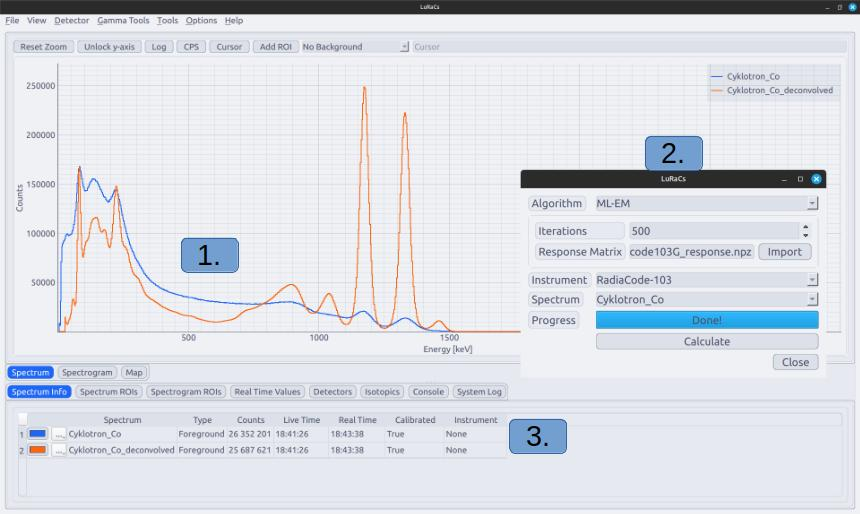
\includegraphics[width = .9\linewidth]{images/interface/gtools_deconvolution.jpg}
    \caption{A Co-60 spectrum deconvolved using ML-EM and a response matrix for a Radiacode-103G detecting a parallel beam of monoenergetic photons.}
    \label{fig:gtools_deconvolution}
    \begin{flushleft}
        \begin{enumerate}
            \item The original Co-60 spectrum  in blue and the deconvolved spectrum in orange.
            \item Control window for the deconvolution operation, see \autoref{tab:gtools_deconvolution}.
            \item The deconvolved spectrum is added as new spectrum, copying information from the original.
        \end{enumerate}
    \end{flushleft}
\end{figure}

\begin{table}[H]
    \centering
    \caption{Description of the deconvolution window.}
    \label{tab:gtools_deconvolution}
    \begin{tabular}{p{.3\textwidth}p{.64\textwidth}}
    \toprule
    \textbf{Field} & \textbf{Description} \\ \midrule
        Algorithm & Which algorithm should be used. Options are \texttt{ML-EM} (use this) and \texttt{Generalized Richardson-Lucy}. \\
        Iterations & The number of iterations the algorithm should run. \\
        (ML-EM) Response Matrix & The path to a .npz file containing the detector response matrix to be used. \\
        Instrument & Instrument providing information for the algorithm. For instance, \texttt{Generalized Richardson-Lucy} is based on the resolution saved in the instrument. \\
        Spectrum & Which spectrum should the operation be executed on. \\
        \bottomrule
    \end{tabular}
\end{table}
\subsubsection{Efficiency}
The intrinsic efficiency is an important detector property and describes the fraction of photons hitting the detector that is actually detected.
\subsubsection{Peak Features}
The \textit{Peak Features}-tool calculates the expected position of gamma spectrum features from a known photopeak energy. The features can then be marked with lines in the \textit{Spectrum}-tab.

\begin{figure}[H]
    \centering
    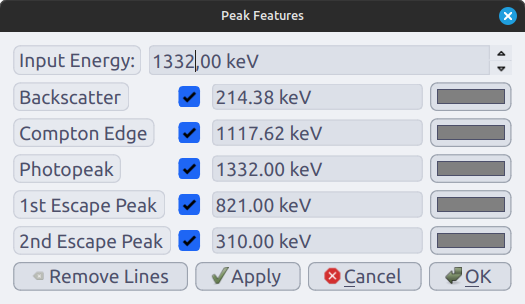
\includegraphics[width = .4\linewidth]{images/interface/peak_features.png}
    \caption{Peak Features tool with the \qty{1332}{\kilo\electronvolt} energy of Co-60 set.}
    \label{fig:peak_features}
    \begin{flushleft}
        \begin{itemize}
            \item \texttt{Remove Lines}: Removed and lines placed in the \textit{Spectrum}-tab.
            \item \texttt{Apply}: Adds lines to the \textit{Spectrum}-tab.
            \item \texttt{Cancel}: Closes the dialog with no other action taken.
            \item \texttt{Ok}: Applies the lines and closes the dialog.
        \end{itemize}
    \end{flushleft}
\end{figure}
\subsubsection{Resolution}
The energy resolution describes how well the detector can resolve detected photons of different energies. A detector with low resolution results in broad peaks which can cover smaller peaks, making them harder to detect.

\begin{figure}[H]
    \centering
    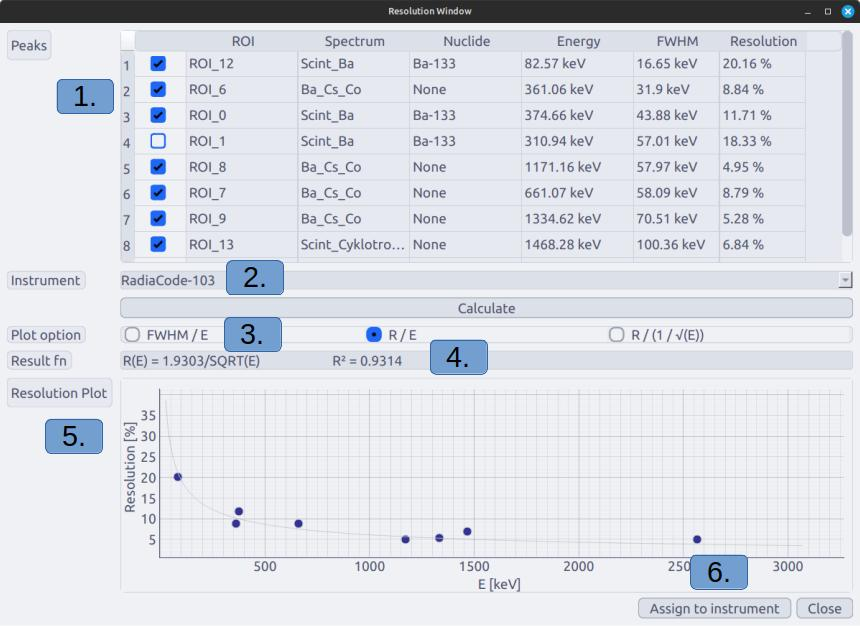
\includegraphics[width = .9\linewidth]{images/interface/gtools_resolution.jpg}
    \caption{Resolution window with several different spectra measured with a 3"x3" NaI(Tl) scintillator loaded. Using \texttt{Tabbed Spectrum View} so the ROIs are only evaluating one spectrum each.}
    \label{fig:gtools_resolution}

    \begin{flushleft}
        \begin{enumerate}
            \item Fitted peaks from all loaded spectra and ROIs. A ROI without a fit can not be included. Unchecked entries will be ignored in the calculation.
            \item Instrument to be given the calculation result. Can be Unique or Generic.
            \item Options for how the calculation results should be plotted. These do not affect the results, only the view.
            \item The resolution function, coefficients are in arbitrary units and not \% (\% = au * 100). The $R^2$ value of the fitted function compared with the data points.
            \item Assign the calculation resolution calibration to the instrument set in (2.).
        \end{enumerate}
    \end{flushleft}
\end{figure}

\subsection{Detector Connection \& Control}
Connecting detectors using the GUI is facilitated through a dialog for each type of connection, they are found under \texttt{Detector -> Connect Bluetooth/USB/Network}. Connecting via Bluetooth or USB requires the application to scan for available devices. The serial number of the connected devices are then displayed, allowing the user to select the appropriate device.
Connecting to network devices requires knowing the IP address and type of the device. Connecting to network detectors have the unique option to use the detector as a GPS. At the moment, this is primarily intended for the Ortec Detective X which has a built in GPS.
When connecting to serial GPS devices the application scans serial ports and lists suggestions. The port can also be entered manually. The baud rate is typically 4800 but a selection of other common rates are also available.

Connecting the a network devices requires knowing the device IP and type beforehand. Connecting to network detectors have the unique option to use the detector as a GPS. This is primarily intended for the Ortec Detective X which has a built in GPS.

When connecting to serial GPS devices the application scans serial ports and lists suggestions but the port can also be entered manually. The baud rate is typically 4800 but a selection of other common rates are also presented.
\subsection{Data Library}\label{sec:data_store}
The \textit{Data Library} allows for saving data objects in the application it self for easy access. It also allows for limited editing of previously saved objects. It contains the following object types \textit{Spectra}, \textit{Spectrograms}, \textit{ROIs}, \textit{Unique Instruments} and \textit{Generic Instruments}. 

All data items saved in the Data Library can be exported to a single zip-file, with a specific internal structure (see \ref{}), using \texttt{File -> Export Data Library}. Such a file can be imported with \texttt{File -> Import Data Library}. 

\subsubsection*{Spectrum Library}
\begin{figure}[H]
    \centering
    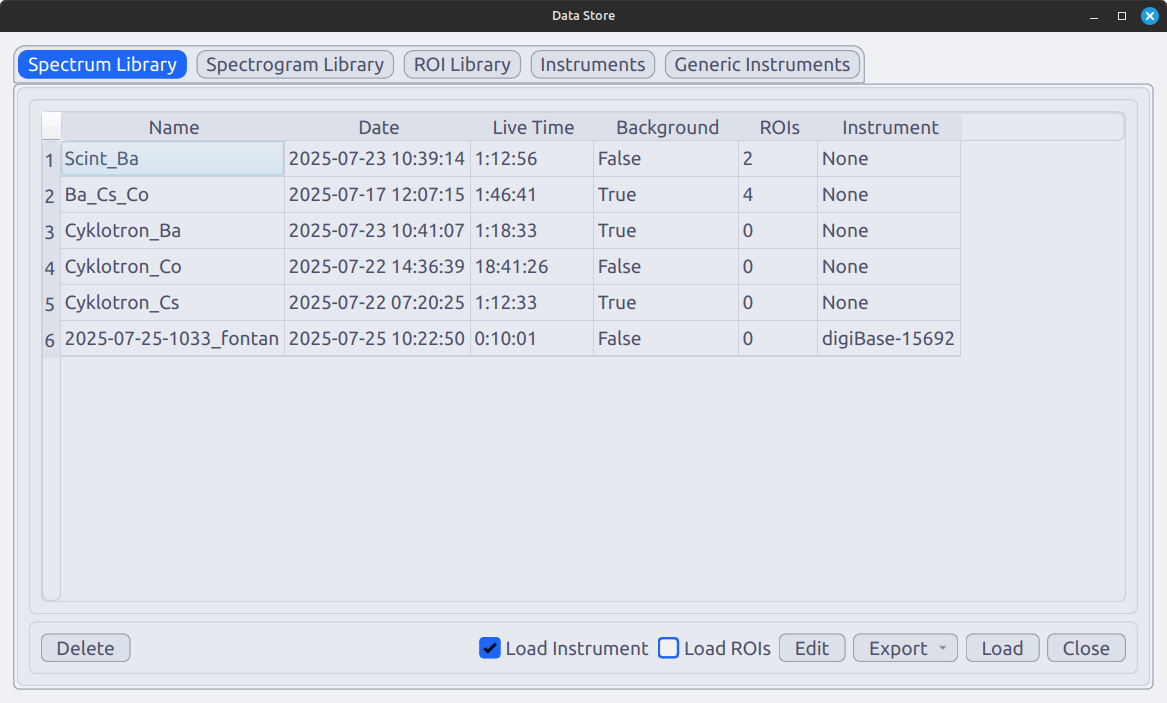
\includegraphics[width = .8\linewidth]{images/interface/data_store_spectrum.png}
    \caption{}
    \label{fig:data_store_spectrum}
\end{figure}

\begin{table}[H]
    \centering
    \caption{Description of the possible operations in toolbar at the bottom of the Spectrum Library-tab}
    \label{tab:spectrum_library_fields}
    \begin{tabular}{p{.3\textwidth}p{.64\textwidth}}
    \toprule
    \textbf{Field} & \textbf{Description} \\ \midrule
    Delete & Remove selected items. \\
    Load Instrument & Load the instrument contained in the specific spectrum file. If not selected LuRaCs will attempt to match the instrument name to an existing \textit{Unique Instrument} save in the Data Library. \\
    Load ROIs & Should the ROIs contained in the spectrum be loaded with the spectrum. \\
    Edit & Edit the spectrum name or remark. \\
    Export & Export the spectrum. Available formats: \texttt{XML}, \texttt{CSV} and \texttt{xlsx}. \\
    Load & Load the spectrum into view. \\
    Close & Close the data Library. \\
    \bottomrule
    \end{tabular}
\end{table}

\begin{table}[H]
    \centering
    \caption{Description of columns in the Spectrum Library-tab}
    \label{tab:spectrum_library_columns}
    \begin{tabular}{p{.3\textwidth}p{.64\textwidth}}
    \toprule
    \textbf{Column} & \textbf{Description} \\ \midrule
    Name & Spectrum name \\
    Date & Date when the measurement of the foreground started \\
    Live Time & Live time of the foreground \\
    ROIs & Number of ROIs saved with the spectrum, if any. \\
    Instrument & Which instrument is saved with the spectrum if any. If an instrument with the same name already exists in the Data Library, it will be used instead of the instrument saved with the spectrum. This can be changed in setting. \\
    \bottomrule
    \end{tabular}
\end{table}

\subsubsection*{Spectrogram Library}
All created spectrograms are placed in the Spectrogram Library. From here they can be loaded back for analysis or continued measurement.
\begin{figure}[H]
    \centering
    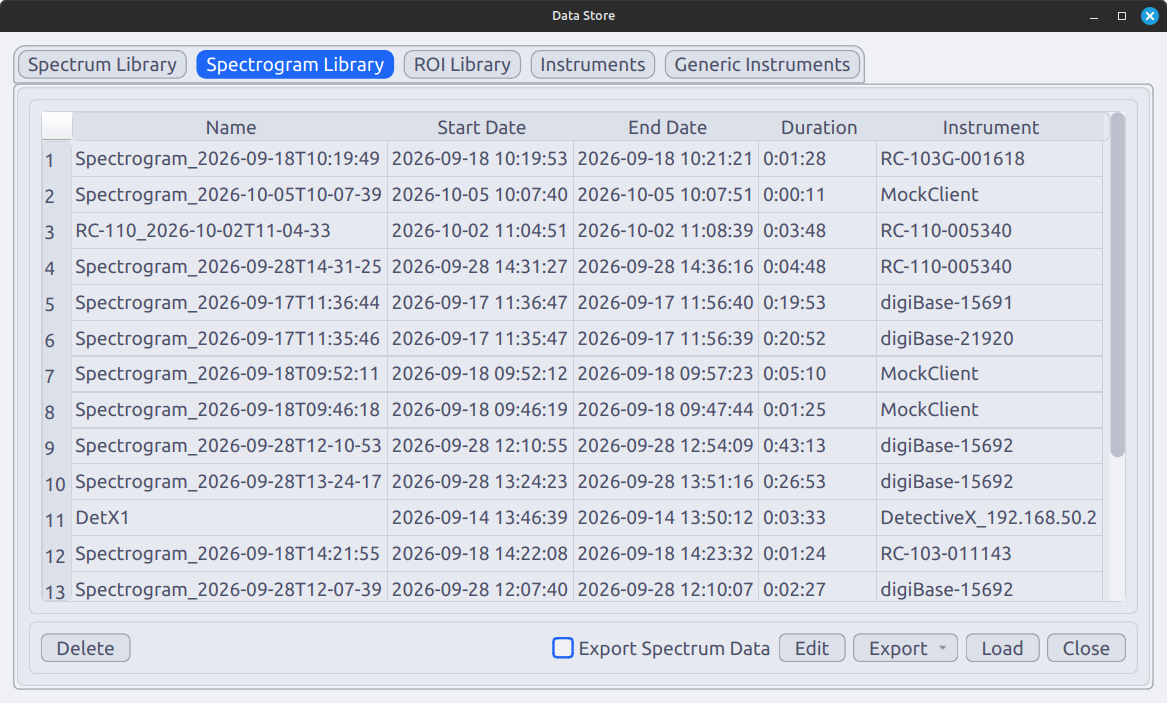
\includegraphics[width = .8\linewidth]{images/interface/data_store_spectrogram.png}
    \caption{}
    \label{fig:data_store_spectrogram}
\end{figure}


\begin{table}[H]
    \centering
    \caption{Description of the possible operations in toolbar at the bottom of the Spectrogram Library-tab}
    \label{tab:spectrogram_library_fields}
    \begin{tabular}{p{.3\textwidth}p{.64\textwidth}}
    \toprule
    \textbf{Field} & \textbf{Description} \\ \midrule
    Delete & Remove selected items. \\
    Export Spectrum Data & If checked the data for  individual channels are included when exporting, everything else is exported the same. \\
    Edit & Edit the spectrogram name. \\
    Export & Export the spectrogram to another file. Available formats: \texttt{.db} (SQLite3) and \texttt{xlsx}. \\
    Load & Load the spectrum into view. \\
    Close & Close the data Library. \\
    \bottomrule
    \end{tabular}
\end{table}

\begin{table}[H]
    \centering
    \caption{Description of columns in the Spectrogram Library-tab}
    \label{tab:spectrogram_library_columns}
    \begin{tabular}{p{.3\textwidth}p{.64\textwidth}}
    \toprule
    \textbf{Column} & \textbf{Description} \\ \midrule
    Name & Spectrogram name \\
    Start Date & Date when the measurement started. \\
    End Date & Date when the measurement was last stopped. \\
    Duration & Total measurement duration. \\
    Instrument & Identifier for the detector used for acquiring the spectrogram. \\
    \bottomrule
    \end{tabular}
\end{table}

\subsubsection*{ROI Library}
The ROI Library allows for saving references to ROIs. These can later be loaded to a spectrum or spectrogram. This means the roi options, like the energy bounds, fitting options and assigned nuclide, are saved but data like fitting parameters and peak counts are not.
\begin{figure}[H]
    \centering
    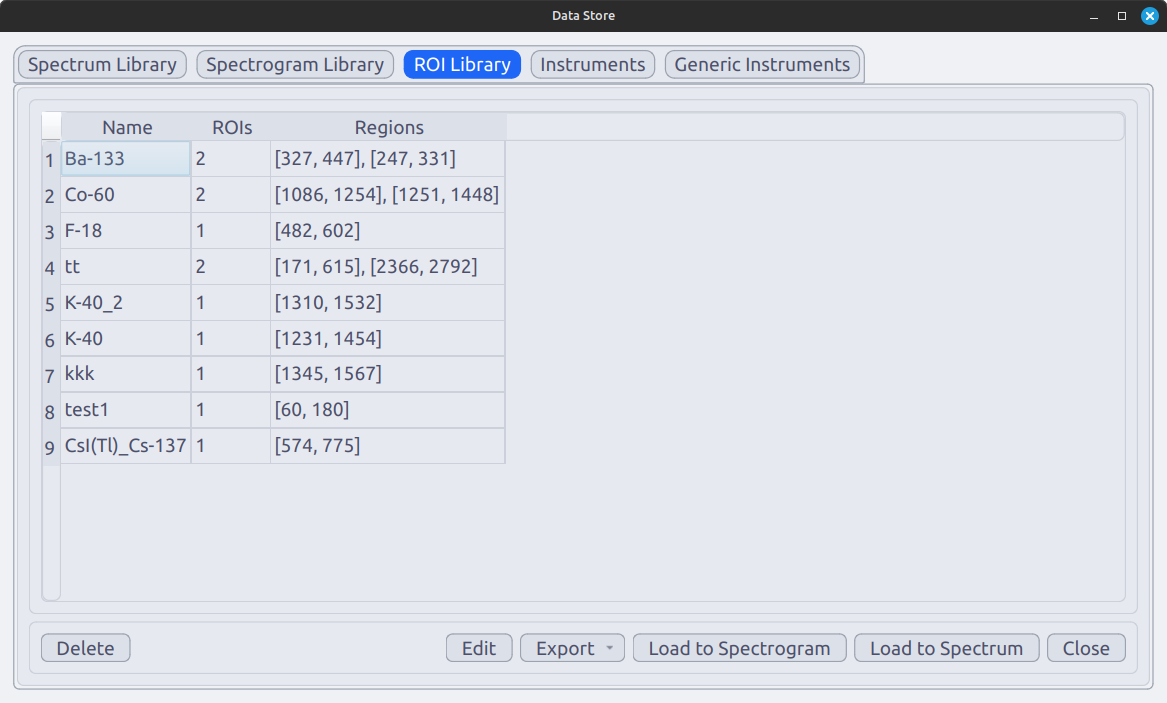
\includegraphics[width = .8\linewidth]{images/interface/data_store_rois.png}
    \caption{}
    \label{fig:data_store_rois}
\end{figure}


\begin{table}[H]
    \centering
    \caption{Description of the possible operations in toolbar at the bottom of the ROI Library-tab}
    \label{tab:roi_library_fields}
    \begin{tabular}{p{.3\textwidth}p{.64\textwidth}}
    \toprule
    \textbf{Field} & \textbf{Description} \\ \midrule
    Delete & Remove selected items. \\
    Edit & Edit the ROI collection name and the ROIs contained within, see \autoref{fig:data_store_roi_edit}. \\
    Export & Export the ROIs to another file. Available formats: \texttt{.xml}. \\
    Load to Spectrogram & Load the ROIs as spectrogram ROIs. \\
    Load to Spectrum & Load the ROIs as spectrum ROIs. \\
    Close & Close the data Library. \\
    \bottomrule
    \end{tabular}
\end{table}

\begin{table}[H]
    \centering
    \caption{Description of columns in the ROI Library-tab}
    \label{tab:roi_library_columns}
    \begin{tabular}{p{.3\textwidth}p{.64\textwidth}}
    \toprule
    \textbf{Column} & \textbf{Description} \\ \midrule
    Name & Name of the ROI group. \\
    ROIs & Number of ROIs in the group. \\
    Regions & The bounds of all ROIs in the group. \\
    \bottomrule
    \end{tabular}
\end{table}

\begin{figure}[H]
    \centering
    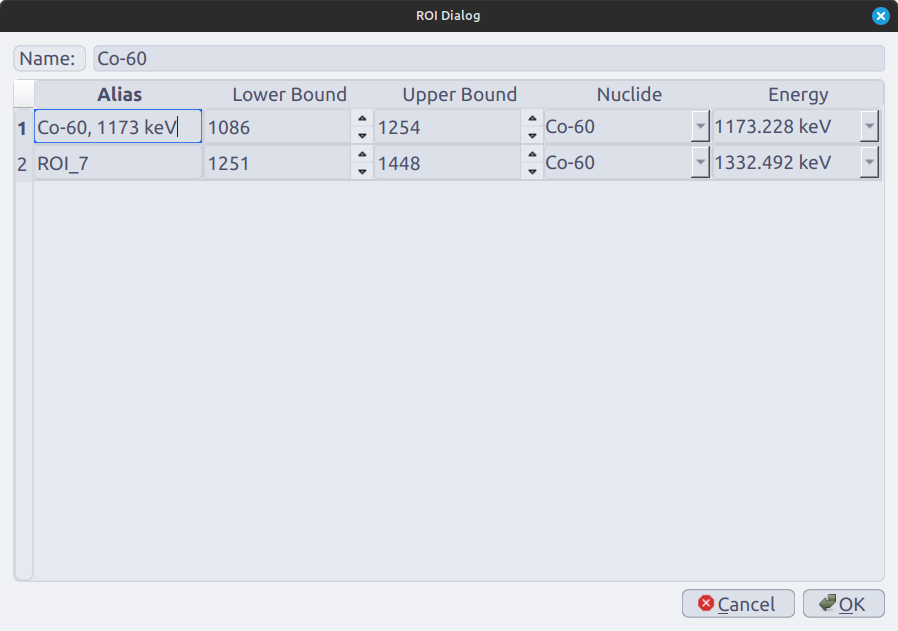
\includegraphics[width = .7\linewidth]{images/interface/data_store_roi_edit.png}
    \caption{ROI editor inside the Data Store. From the nuclide library, it is possible to change the ROI alias/name as well as upper and lower bounds, nuclide, emission.}
    \label{fig:data_store_roi_edit}
\end{figure}

\subsubsection*{Unique-/Generic Instruments}
The tabs for the Unique and Generic Instruments are very similar and therefore described in the same section.
\begin{figure}[H]
    \centering
    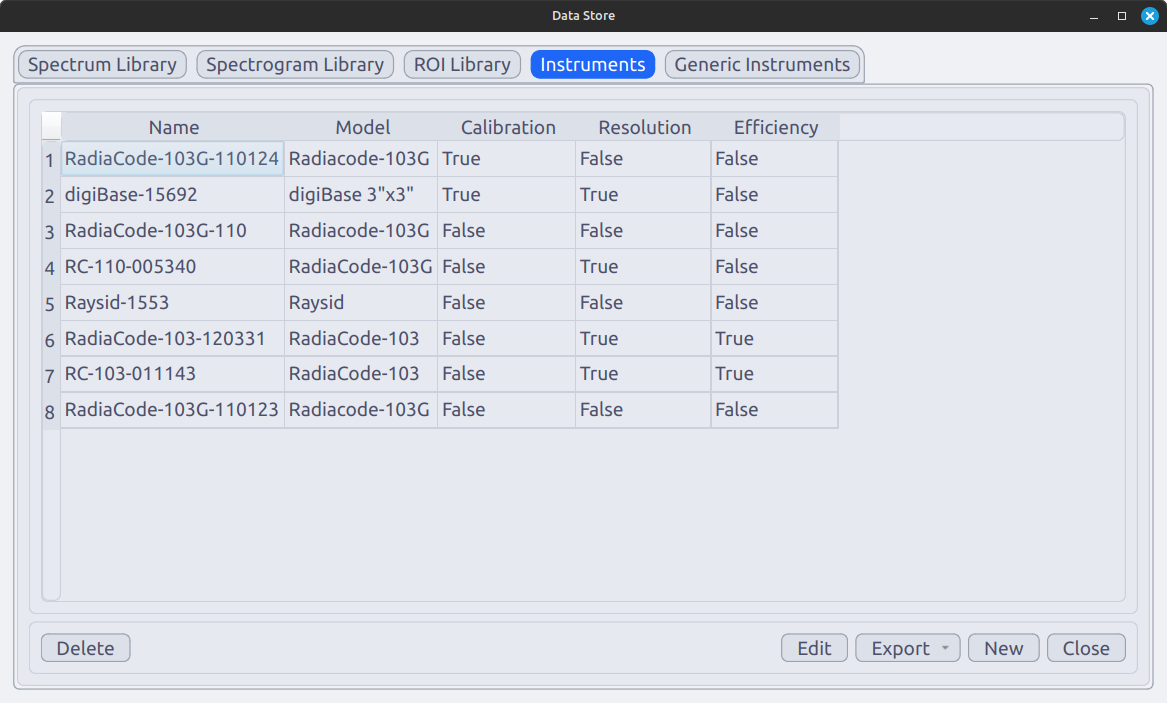
\includegraphics[width = .8\linewidth]{images/interface/data_store_instrument.png}
    \caption{Instruments-tab in the Data Library, with eight listed Unique Instruments.}
    \label{fig:data_store_instruments}
\end{figure}


\begin{table}[H]
    \centering
    \caption{Description of the possible operations in toolbar at the bottom of the Instruments-tab}
    \label{tab:instrument_library_fields}
    \begin{tabular}{p{.3\textwidth}p{.64\textwidth}}
    \toprule
    \textbf{Field} & \textbf{Description} \\ \midrule
    Delete & Remove selected items. \\
    Edit & Edit an existing instrument, see \autoref{fig:data_store_instrument_edit}. \\
    Export & Export the instrument data to another file. Available formats: \texttt{.xml}. \\
    New & Create a new instrument. \textit{Unique Instruments} can inherit data from \textit{Generic Instruments}. \\
    Close & Close the data Library. \\
    \bottomrule
    \end{tabular}
\end{table}

\begin{table}[H]
    \centering
    \caption{Description of columns in the Instruments-tab}
    \label{tab:instrument_library_columns}
    \begin{tabular}{p{.3\textwidth}p{.64\textwidth}}
    \toprule
    \textbf{Column} & \textbf{Description} \\ \midrule
    Name & Instrument name (Only for \textit{Unique Instrument}) \\
    Model & Name of the instrument model. Ex. RadiaCode-110 or Identifinder R400. \\
    Calibration & Shows if the instrument stores an energy calibration. (Only for \textit{Unique Instrument}) \\
    Resolution & Shows if the instrument stores an energy resolution. \\
    Efficiency & Shows if the instrument stores an intrinsic efficiency. \\
    \bottomrule
    \end{tabular}
\end{table}

\begin{figure}[H]
    \centering
    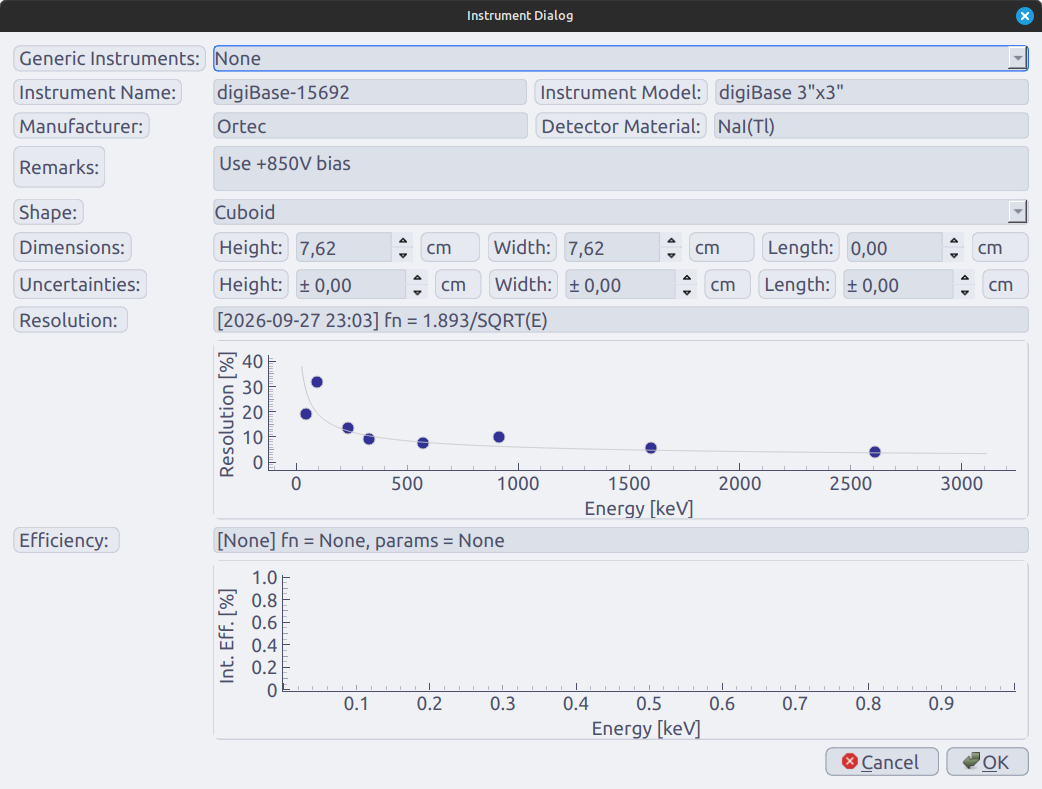
\includegraphics[width = .8\linewidth]{images/interface/data_store_instrument_edit.png}
    \caption{The dialog for creating a new instrument or editing an existing one. 'Instrument Name' can not be changed for a generic instrument.}
    \label{fig:data_store_instrument_edit}
\end{figure}
\subsection{Settings}
The settings are divided into \texttt{Settings} that contain basic and cosmetic settings, and \texttt{Advanced Settings} containing settings that ordinary users rarely need to interact with.

% ============================================================
% General Settings
% ============================================================

\begin{longtable}{p{0.30\textwidth} p{0.62\textwidth}}
    \caption{Application settings.}
    \label{tab:settings} \\

    \hline
    \textbf{Setting} &
    \textbf{Description} \\
    \hline
    \endfirsthead

    \multicolumn{2}{c}%
    {\tablename\ \thetable{} -- continued from previous page} \\
    \hline
    \textbf{Setting} &
    \textbf{Description} \\
    \hline
    \endhead

    \hline
    \multicolumn{2}{r}{Continued on next page} \\
    \endfoot

    \hline
    \endlastfoot

    % ------------------------------------------------------------
    % Appearance
    % ------------------------------------------------------------

    \multicolumn{2}{l}{\textbf{Appearance}} \\

    Theme &
        Select the visual theme used by the application interface and plots. \\

    Plot Colour Scheme &
        Select the color scheme used when automatically assigning colors to plotted spectra. Options are \textit{MatplotLib}, \texttt{LibreOffice} and \texttt{Catppuccin} \\

    Spectrum Draw Style &
        Select how spectra are rendered. Available options are
        \emph{Pen}, \emph{Brush}, and \emph{Pen + Brush}. \\

    Font Size &
        Set the application font size in points. \\

    Spectrum Plot xMax &
        Set the maximum energy displayed on spectrum plots, in keV. \\

    Verbose Calculation Logging &
        Enable additional logging during calculations. This can be useful
        when diagnosing calculation or processing problems. \\

    % ------------------------------------------------------------
    % Import Options
    % ------------------------------------------------------------

    \multicolumn{2}{l}{\textbf{Import Options}} \\

    Load ROIs on import &
        Automatically load regions of interest when importing a spectrum from a file. \\

    Load instrument on import &
        Automatically load instrument information when importing a spectrum from a file. \\

    Load calibration from instrument &
        Load the energy calibration associated with the instrument when
        importing data from the Data Store or from a file. \\

\end{longtable}


% ============================================================
% Advanced Settings
% ============================================================

\begin{longtable}{p{0.30\textwidth} p{0.62\textwidth}}
    \caption{Advanced application settings.}
    \label{tab:advanced-settings} \\

    \hline
    \textbf{Setting} &
    \textbf{Description} \\
    \hline
    \endfirsthead

    \multicolumn{2}{c}%
    {\tablename\ \thetable{} -- continued from previous page} \\
    \hline
    \textbf{Setting} &
    \textbf{Description} \\
    \hline
    \endhead

    \hline
    \multicolumn{2}{r}{Continued on next page} \\
    \endfoot

    \hline
    \endlastfoot

    % ------------------------------------------------------------
    % Device Running
    % ------------------------------------------------------------

    \multicolumn{2}{l}{\textbf{Device Running}} \\

    Update Loop Delay &
        Set the delay between iterations of the device monitoring and update
        loop, in seconds. \\

    Spectrum Update Delay &
        Set the delay between spectrum updates during live acquisition,
        in seconds. \\

    % ------------------------------------------------------------
    % Device Scanning
    % ------------------------------------------------------------

    \multicolumn{2}{l}{\textbf{Device Scanning}} \\

    GUI Scan Length &
        Set the duration of Bluetooth Low Energy scans initiated through
        the graphical user interface, in seconds. \\

    Headless Scan Length &
        Set the duration of Bluetooth Low Energy scans when no the scan is not tracked in the GUI, in seconds. \\

    % ------------------------------------------------------------
    % Optimizer
    % ------------------------------------------------------------

    \multicolumn{2}{l}{\textbf{Optimizer}} \\

    Optimizer Max Iter &
        Set the maximum number of iterations allowed by the optimizer. \\

    Optimizer Tolerance &
        Set the convergence tolerance used by the optimizer. \\

    Use Chi$^2$ Weight &
        Enable $\chi^2$ weighting during optimization. \\

    % ------------------------------------------------------------
    % Logging
    % ------------------------------------------------------------

    \multicolumn{2}{l}{\textbf{Logging}} \\

    Log Exceptions &
        Enable logging of unhandled exceptions. \\

    Write logs to file &
        Enable writing log messages to the application log file. \\

    Write logs to console &
        Enable writing log messages to the terminal or console. \\

    Headless Log Buffer Length &
        Set the maximum number of log entries retained in the in-memory
        log buffer. Changes to this setting require an application restart. \\

    % ------------------------------------------------------------
    % Spectrogram
    % ------------------------------------------------------------

    \multicolumn{2}{l}{\textbf{Spectrogram}} \\

    Spectrogram View Buffer &
        Set the number of recent spectrogram data points retained for
        display. \\

    % ------------------------------------------------------------
    % Maps
    % ------------------------------------------------------------

    \multicolumn{2}{l}{\textbf{Maps}} \\

    Save extra GPS data &
        Enable saving additional GPS information with map-related data. \\

\end{longtable}
\subsection{Command Line Arguments}
Command Line Arguments can be provided when starting the application from a terminal. 
% ============================================================
% Command-Line Options
% ============================================================

\begin{longtable}{p{0.34\textwidth} p{0.58\textwidth}}
    \caption{Command-line options available when starting LuRaCs.}
    \label{tab:cli-options} \\

    \hline
    \textbf{Option} &
    \textbf{Description} \\
    \hline
    \endfirsthead

    \multicolumn{2}{c}%
    {\tablename\ \thetable{} -- continued from previous page} \\
    \hline
    \textbf{Option} &
    \textbf{Description} \\
    \hline
    \endhead

    \hline
    \multicolumn{2}{r}{Continued on next page} \\
    \endfoot

    \hline
    \endlastfoot

    % ------------------------------------------------------------
    % General
    % ------------------------------------------------------------

    \multicolumn{2}{l}{\textbf{General}} \\

    \texttt{--debug} &
        Launch the application in debug mode. A mock device is added
        automatically for testing and development. \\

    \texttt{--headless} &
        Run the application without the graphical user interface,
        using terminal mode instead. \\

    \texttt{--clear\_local\_cache} &
        Remove all locally stored files and exit the application. \\

    % ------------------------------------------------------------
    % Data Import
    % ------------------------------------------------------------

    \multicolumn{2}{l}{\textbf{Data Import}} \\

    \texttt{--import\_spectrum <file> [file ...]} &
        Load one or more spectrum files when starting the application.
        Each specified file must exist and be supported by the
        application's file importer. \\

    \texttt{--import\_rois <file>} &
        Load regions of interest from the specified XML file. \\

    \texttt{-roi <lower> <upper>} &
        Add a region of interest with the specified lower and upper
        energy bounds in keV. The option can be specified multiple
        times to add several ROIs. \\

    \texttt{--nuclides <nuclide> [nuclide ...]} &
        Preset one or more nuclides in the isotopics interface.
        This option is applied when the graphical user interface is
        available. \\

    % ------------------------------------------------------------
    % Device Connections
    % ------------------------------------------------------------

    \multicolumn{2}{l}{\textbf{Device Connections}} \\

    \texttt{-ble <device> [device ...]} &
        Attempt to establish Bluetooth Low Energy connections using
        the specified device names. \\

    \texttt{--bluetooth <device> [device ...]} &
        Long-form alias for \texttt{-ble}. Attempts Bluetooth Low
        Energy connections using the specified device names. \\

    \texttt{-usb <device> [device ...]} &
        Attempt to establish USB connections using the specified
        device names. Matching is performed against detected USB
        device product names. \\

    \texttt{-nw <ip> [ip ...]} &
        Attempt to connect to network devices using their IP addresses. \\

    \texttt{--network <ip> [ip ...]} &
        Long-form alias for \texttt{-nw}. Connects to network devices
        using their IP addresses. \\

    \texttt{--serial\_gps <interface>} &
        Connect a GPS receiver using a USB serial interface. The
        specified value identifies the serial interface used by
        the GPS receiver. \\

    % ------------------------------------------------------------
    % Maps
    % ------------------------------------------------------------

    \multicolumn{2}{l}{\textbf{Maps}} \\

    \texttt{--map\_url <URL>} &
        Load an online map from the specified URL at application startup. Only one map source may be specified at startup. \\

    \texttt{--map\_file <path>} &
        Load a local offline map from the specified \texttt{.pmtiles}
        file at application startup. Only one map source may be specified at startup. \\

\end{longtable}

\subsection{Command Line Interface (CLI)}\label{subsec:cli}
LuRaCs is primarily operated through the GUI but it also provides a terminal-based command line interface, allowing for controlling detectors without a GUI. This may be useful if remote measurements or measurements run on a Raspberry Pi is attached to a drone. This mode shares most of the same commands as the GUI Console with the exception of visualisation tools.

This mode is started by running LuRaCs in a terminal with the \texttt{--headless} flag.

\begin{figure}[H]
    \centering
    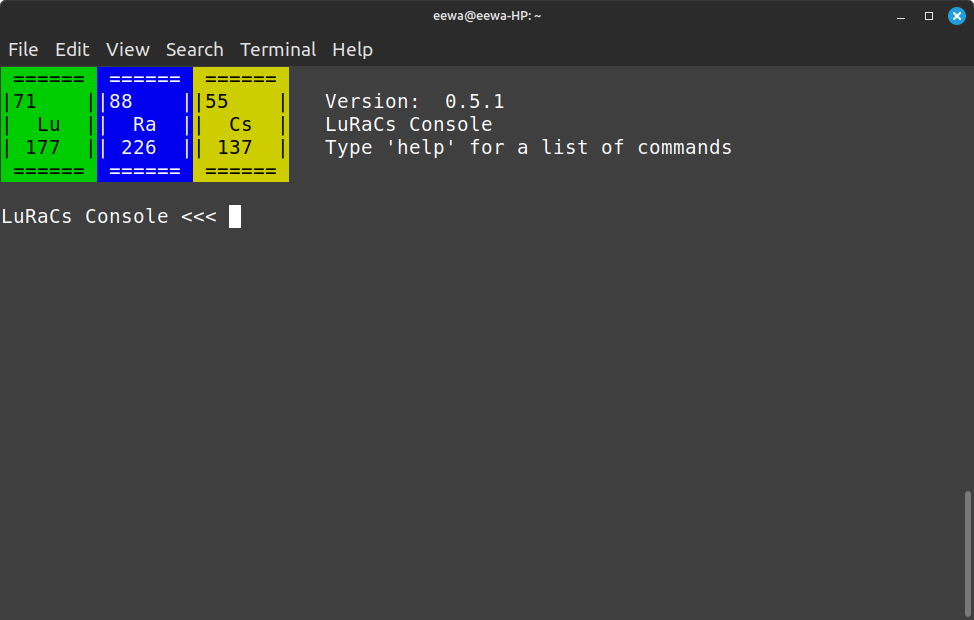
\includegraphics[width = .8\linewidth]{images/interface/cli.png}
    \caption{LuRaCs command line interface in terminal mode.}
    \label{fig:cli}
\end{figure}

\begin{figure}[H]
    \centering
    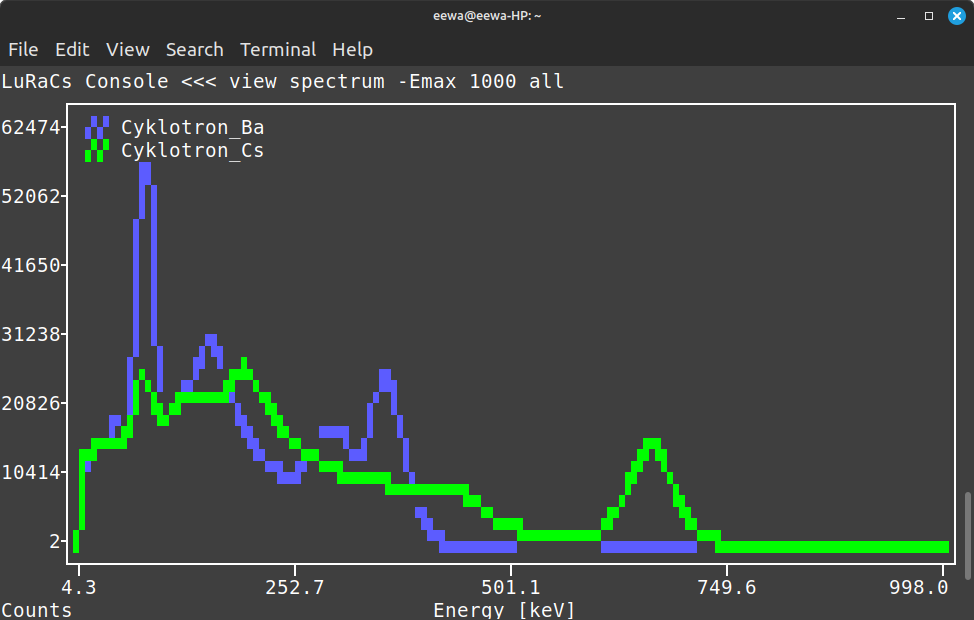
\includegraphics[width = .8\linewidth]{images/interface/cli_spectrum.png}
    \caption{Two spectra viewed through the command line using the command \texttt{view spectrum -Emax 1000 all}. The \texttt{-Emax 1000} flag limits the x-axis to $< 1000$ keV.}
    \label{fig:cli_spectrum}
\end{figure}

%---------------------------------------------------------------
% Command Reference
% ----------------------------------------------------------------

\begin{longtable}{>{\ttfamily}p{0.38\textwidth} p{0.55\textwidth}}
    \caption{Command-line interface command reference.}
    \label{tab:command-reference} \\

    \hline
    \textnormal{\textbf{Command}} &
    \textnormal{\textbf{Description}} \\
    \hline
    \endfirsthead

    \multicolumn{2}{c}%
    {\tablename\ \thetable{} -- continued from previous page} \\
    \hline
    \textnormal{\textbf{Command}} &
    \textnormal{\textbf{Description}} \\
    \hline
    \endhead

    \hline
    \multicolumn{2}{r}{Continued on next page} \\
    \endfoot

    \hline
    \endlastfoot

    % ============================================================
    % General
    % ============================================================

    \multicolumn{2}{l}{\textbf{General}} \\
    \texttt{help} &
        Display the available commands and their descriptions. \\

    \texttt{clear} &
        Clear the console and return the application to start. \\

    \texttt{exit}, \texttt{quit}, \texttt{shutdown} &
        Exit the application. \\

    \hline

    % ============================================================
    % Device Management
    % ============================================================

    \multicolumn{2}{l}{\textbf{Device Management}} \\

    \texttt{device scan usb} &
        Scan for connected USB devices. \\

    \texttt{device scan ble} &
        Scan for nearby Bluetooth Low Energy devices. \\

    \texttt{device connect usb <device>} &
        Connect to a USB device matching the specified name. \\

    \texttt{device connect ble <device1> [device2 ...]} &
        Connect to one or more Bluetooth Low Energy devices. \\

    \texttt{device disconnect <device>} &
        Disconnect the specified device. \\

    \texttt{device disconnect all} &
        Disconnect all connected devices. \\

    \hline

    % ============================================================
    % Resource Listing
    % ============================================================

    \multicolumn{2}{l}{\textbf{Resource Listing}} \\

    \texttt{list devices} &
        Display all connected devices. \\

    \texttt{list spectra} &
        Display all loaded spectra. \\

    \texttt{list spectrogram} &
        Display all loaded spectrograms. \\

    \texttt{list rois} &
        Display all loaded regions of interest. \\

    \hline

    % ============================================================
    % Indexes
    % ============================================================

    \multicolumn{2}{l}{\textbf{Indexes}} \\

    \texttt{index spectrum} &
        Display indexed spectrum files. \\

    \texttt{index spectrogram} &
        Display indexed spectrogram files. \\

    \texttt{index roi} &
        Display indexed ROI files. \\

    \hline

    % ============================================================
    % Viewing
    % ============================================================

    \multicolumn{2}{l}{\textbf{Viewing Data}} \\

    \texttt{view spectrum <name>} &
        Display the specified spectrum. The spectrum can be selected by name
        or by its index in the loaded spectrum list. \\

    \texttt{view spectrum -n <name>} &
        Specify the spectrum to display by name. \\

    \texttt{view spectrum all} &
        Display all loaded spectra on the same plot. \\

    \texttt{view spectrum -A} &
        Display all loaded spectra on the same plot. \\

    \texttt{view spectrum -Emin <energy>} &
        Set the lower energy limit of the displayed spectrum, in keV. \\

    \texttt{view spectrum -Emax <energy>} &
        Set the upper energy limit of the displayed spectrum, in keV. \\

    \texttt{view spectrum -cps} &
        Display the spectrum as counts per second (CPS) instead of total
        counts. \\

    \texttt{view spectrum -log} &
        Display the spectrum using the logarithmic scaling. \\

    \texttt{view spectrum -bkgSub} &
        Display the background-subtracted spectrum, if the spectrum has a background. \\

    \texttt{view rois} &
        Display the currently loaded regions of interest. \\

    \texttt{view log} &
        Display recent application log entries. \\

    \hline

    % ============================================================
    % ROI
    % ============================================================

    \multicolumn{2}{l}{\textbf{ROI Management}} \\

    \texttt{roi <lower> <upper>} &
        Add a region of interest between the specified lower and upper
        bounds. \\

    \texttt{roi -c} &
        Clear all regions of interest. \\

    \hline

    % ============================================================
    % Spectrogram
    % ============================================================

    \multicolumn{2}{l}{\textbf{Spectrogram Management}} \\

    \texttt{spectrogram start <device>} &
        Start a spectrogram for the specified device. \\

    \texttt{spectrogram start all} &
        Start spectrograms for all connected devices. \\

    \texttt{spectrogram pause <name>} &
        Pause the specified spectrogram. \\

    \texttt{spectrogram pause all} &
        Pause all running spectrograms. \\

    \texttt{spectrogram unpause <name>} &
        Resume the specified spectrogram. \\

    \texttt{spectrogram unpause all} &
        Resume all paused spectrograms. \\

    \texttt{spectrogram load <path>} &
        Load a spectrogram from the specified file. \\

    \texttt{spectrogram unload <name>} &
        Unload the specified spectrogram. \\

    \texttt{spectrogram unload all} &
        Unload all loaded spectrograms. \\

    \texttt{-n <name>} &
        Specify a custom name when starting a spectrogram. \\

    \texttt{-i <seconds>} &
        Set the spectrogram save interval. Default: $1$ second. \\

    \texttt{-c <count>} &
        Set the number of spectra to concatenate before saving.
        Default: $1$. \\

    \hline

    % ============================================================
    % Maps
    % ============================================================

    \multicolumn{2}{l}{\textbf{Map Management}} \\

    \texttt{map url <https-URL>} &
        Load an online map from the specified HTTPS URL. \\

    \texttt{map file <path>} &
        Load a local offline map from a PMTiles file. \\

    \hline

    % ============================================================
    % Monitoring
    % ============================================================

    \multicolumn{2}{l}{\textbf{Monitoring}} \\

    \texttt{watch} &
        Continuously display live information from connected devices.
        Press \texttt{Ctrl+C} to stop. \\

    \hline

    % ============================================================
    % Automation
    % ============================================================

    \multicolumn{2}{l}{\textbf{Automation}} \\

    \texttt{exec <script-file>} &
        Execute commands from a script file. Empty lines and lines
        beginning with \texttt{\#} are ignored. \\

\end{longtable}
